\documentclass[10pt]{article}
% Anonymous submission by default. preprint.tex defines \PREPRINT and inputs this file to build the
% de-anonymised version (author, repository link) for arXiv.
\ifdefined\PREPRINT
  \usepackage[preprint]{tmlr}
\else
  \usepackage{tmlr}
\fi

\usepackage{amsmath,amssymb}
\usepackage{graphicx}
\usepackage{booktabs}
\usepackage{multirow}
\usepackage{array}
\usepackage{xcolor}
\usepackage{url}
\usepackage[hidelinks]{hyperref}
\usepackage{etoolbox}
\AtBeginEnvironment{table}{\setlength{\belowcaptionskip}{6pt}}  % a line of space between a table's caption and its rule

\graphicspath{{figures/}}

% ---------------------------------------------------------------- macros
\newcommand{\Neff}{N_{\mathrm{eff}}}
\newcommand{\Nonce}{N_{\mathrm{once}}}
\newcommand{\Nrec}{N_{\mathrm{rec}}}
\newcommand{\Nstar}{N^{\star}}
\newcommand{\tpp}{tokens per parameter}
\newcommand{\lbl}[1]{\textit{#1}}          % evidence labels: pre-registered / pre-specified / exploratory
\ifdefined\PREPRINT
  \hypersetup{pdftitle={What a Loop Buys: Parameter Efficiency on Text, Extendable Depth on a Serial Task},
               pdfauthor={Qirun Li}}
  \newcommand{\coderepo}{\url{https://github.com/bethehand/looped-scaling}}
  \newcommand{\theauthors}{the author}
\else
  \newcommand{\coderepo}{an anonymised repository (link in the supplementary material)}
  \newcommand{\theauthors}{the authors}
\fi

\title{What a Loop Buys: Parameter Efficiency on Text,\\Extendable Depth on a Serial Task}

\author{\name Qirun Li \email qli858246@gmail.com \\
      \addr Independent researcher}

\def\month{MM}
\def\year{YYYY}
\def\openreview{\url{https://openreview.net/forum?id=XXXX}}

\begin{document}

\maketitle

\begin{abstract}
When does running a block of layers again work as test-time compute? A looped transformer adds depth without adding
parameters, and two benefits are claimed for it: that it behaves like a larger model, and that more loops at inference
solve harder problems without a written chain of thought. We test both: on web text in a pre-registered study, and on a
synthetic serial task whose design and predictions were frozen before its main runs. On web text we
trained a grid of 111 models from 10M to 80M parameters with dense references up to 160M, varying where the loop sits,
how often it runs and how it is backpropagated, and extended it in model size, data and learning rate. On a
lookup-chain task that needs serial steps we compared looped models with dense models of equal parameters and of
equal executed depth, with a written chain of thought and with pause tokens. None of the four pre-registered
hypotheses held as stated, and the pre-registered effective-parameter exponent is not identified. In an exploratory
analysis without a fitted law, each parameter of a model whose middle block is looped 4 times is worth at most about
one dense parameter at 10--20M with up to 20 training tokens per parameter and about 1.3--1.5 at 40M--160M with 20--40,
rising with the tokens per parameter; at equal training compute and a shared learning rate the dense model wins every measured comparison, by a
margin that shrinks with data. On text the
looped block runs a fixed-length program, a cycle or a fixed point, depending on training, and gains nothing from
extra loops. On the chain task the same architecture computes the chain step by step inside the loop and solves
longer chains when run longer (a model trained with 8 loops on chains of at most 8 steps goes from 0.04 to 0.83
accuracy on 12-step chains when run with 16 loops), and for most training regimes its own confidence tells it when to
stop. Dense models of
equal depth do not extend beyond the training range, and neither does a chain of thought on this task, whose prompt
grows with the chain. At deployment and equal loss, a middle block looped 4 times saves at most 19\% of the weight
memory and costs about 2.2--2.5 times the KV cache and the decoding time. Code, configurations, training logs and results are released.
\end{abstract}

\section{Introduction}
\label{sec:intro}

A looped, or recurrent-depth, transformer applies one block of layers several times in a row
\citep{dehghani2019universal,geiping2025scaling,zhu2025scaling}. Running a block $r$ times costs $r$ times its
compute and adds no parameters. Two benefits are expected in return. The first is \emph{parameter efficiency}: a
looped model should behave like a larger dense model, which matters wherever memory or bandwidth rather than
arithmetic limits deployment. The second is \emph{latent reasoning}: if the loop iterates on a problem, running more
loops at inference should solve harder problems without writing out a chain of thought, a form of test-time compute
that lives inside the network.

Both claims are hard to check from the literature. Studies differ in data, tokenizer, training recipe and model
family; seeds are rarely reported; and the quantity of interest, how much one more loop is worth, is usually read off
a single fitted scaling law \citep{schwethelm2026how,prairie2026parcae,chen2026moe}. Evidence for test-time scaling
comes from two directions that are seldom put side by side: large models trained with a random number of loops, which
become robust to the loop count \citep{geiping2025scaling}, and small models on algorithmic tasks, which solve longer
problems when run longer \citep{fan2025looped,kohli2026loop,zhang2026recurrence}.

We measured both claims in one study, with one architecture family and one recipe, and with the hypotheses and the
analysis written down before the first training run. On web text, a grid of 111 runs varies model size (10M to 80M
looped, dense references to 160M), where the loop sits (a middle block or the whole stack), how often it runs ($r$ =
2, 4, 8) and how it is backpropagated (through all loops or through the last half), with three seeds at the small
sizes and cooldown branches at three data budgets. Extensions add a 160M looped model, up to 160 training tokens per
parameter, random loop counts, and nine supplementary experiments whose plans were frozen before they ran. When the
text results left the second claim untested, we built a task that needs serial steps, a chain of lookups in fixed
random tables, froze its design and predictions, and ran it the same way: looped models against dense models of equal
parameters and of equal executed depth, against a dense model that writes the chain out, and against pause tokens.

\begin{figure}[t]
  \centering
  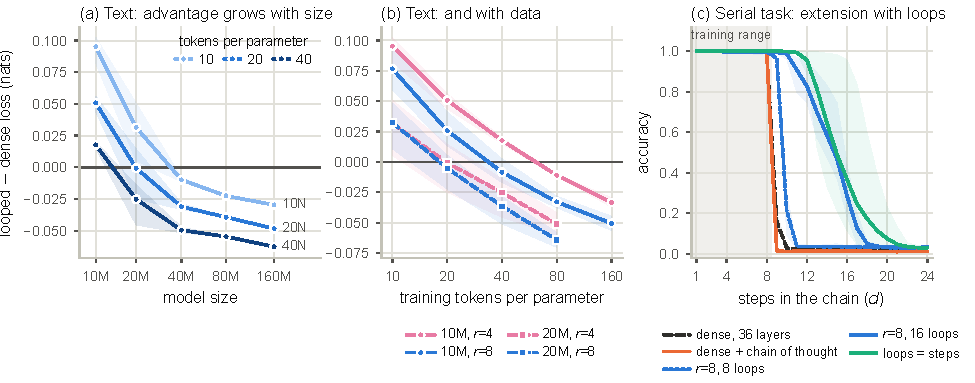
\includegraphics[width=\linewidth]{fig1_overview}
  \caption{What a loop buys, in one figure. \textbf{(a)}~On web text, at equal parameters and training tokens, a
  middle block looped 4 times goes from worse than the dense model at 10M to better at every budget from 40M on
  (looped minus dense validation loss; budgets of 10, 20 and 40 training tokens per parameter; band: range over
  seeds). \textbf{(b)}~The advantage also grows with the training tokens per parameter, here at 10M and 20M for
  middle blocks looped 4 and 8 times. \textbf{(c)}~On chains of table lookups, trained on 1--8 steps (shaded), dense
  models of the same executed depth stop at the training range, and so does a dense model that writes the chain out,
  whose prompt grows with the chain; a looped model run with more loops than in training solves longer chains (mean over
  five seeds; band: range).}
  \label{fig:overview}
\end{figure}

The two settings give different answers (Figure~\ref{fig:overview}). On text, the loop buys parameter and data
efficiency, not compute efficiency: measured without a fitted law, a parameter of the looped block is worth at most
about one dense parameter at 10--20M with up to 20 training tokens per parameter and about 1.3--1.5 dense parameters
at 40M--160M, the value grows with the tokens per parameter, and at equal training compute the dense model wins every
comparison we could measure, by a margin that shrinks with data. Depending on how it is trained, the looped block
runs a fixed-length program, a cycle or a fixed point, and none of these gains from extra loops at inference. On the
chain task, the same architecture computes the chain step by step inside the loop, solves chains longer than it was
trained on when run longer, and for most training regimes can tell from its own confidence when to stop. A written
chain of thought is perfect within the training range at a third of the compute and does not extend at all; on this
task, whose prompt grows with the chain, that is a failure to generalise to longer inputs.

We read the difference as a matter of three conditions, which the chain task meets once the model is trained for
them: \emph{headroom}, meaning that errors come from too few serial steps rather than from missing knowledge;
\emph{extendable iteration}, meaning that the loop can run longer without destroying its state; and a \emph{stopping
signal}. On web text at these sizes we saw no sign of the first. This reading is an interpretation of two settings,
not a tested law, and Section~\ref{sec:discussion} discusses what would test it.

Our contributions are:
\begin{itemize}
  \item \textbf{A pre-registered measurement of what a loop is worth on text} (Section~\ref{sec:text}). None of the four
  hypotheses held as stated. The pre-registered exponent $\varphi$ of the effective-parameter law
  $\Neff = \Nonce + r^{\varphi}\Nrec$ is not identified, because the dense law it is read from is weakly identified.
  Measured without that law, the value of a loop depends on model size and on training tokens per parameter, an
  interaction that effective-parameter laws with one exponent per architecture do not capture. At equal training
  compute the dense model wins all 258 measured comparisons, up to 640 tokens per parameter, and the two reach parity
  only at the smallest size and the most data, with the looped model's own learning rate.
  \item \textbf{What the looped block computes on text} (Section~\ref{sec:mechanism}). Depending on training, it runs
  a fixed-length program, a periodic cycle or a contraction to a fixed point; none gains from extra loops.
  \item \textbf{Loops as extendable depth on a serial task} (Section~\ref{sec:serial}). With dense controls of equal
  executed depth and probes of every intermediate value, looped models compute the chain step by step (one step per
  loop when the model has a loop for every step) and solve longer chains with more loops at inference.
  The learning rate decides whether this is learned at all. In a controlled comparison of answer-free stopping rules,
  the model's own confidence is the best rule that actually stops, and a training regime with a few random extra loops
  gives a model that both extends and stops.
  \item \textbf{A comparison with reasoning written out} (Section~\ref{sec:cot}). On this task, a dense model that
  writes the chain out as tokens is perfect within the training range and fails beyond it from the first written token
  on, a failure to generalise to longer prompts that leaves open what happens when the input length is fixed. Pause
  tokens add nothing.
  \item \textbf{The cost at deployment} (Section~\ref{sec:cost}), and an open record: the pre-registration, a dated log
  of every deviation and correction, and the results and training logs of all 232 language-model runs and 135
  synthetic-task runs (Section~\ref{sec:process}).
\end{itemize}

\section{Related work}
\label{sec:related}

\paragraph{How much a loop is worth.}
Sharing parameters across layers is an old way to trade compute for parameters
\citep{dehghani2019universal,lan2019albert,bae2025relaxed}. \citet[App.~D.2, Fig.~17]{kaplan2020scaling} found that transformers
which re-use parameters ``perform slightly better when comparing models with equal parameter count, but slightly worse
when accounting for reuse and comparing per FLOP''; our results agree in both directions and add how the balance moves
with model size and data. The effective-parameter form we test, $\Neff = \Nonce + r^{\varphi}\Nrec$, and our choice
of two unshared layers before and after the loop come from \citet{schwethelm2026how}, who estimate $\varphi = 0.46$
(95\% interval 0.41--0.53) on FineWeb-Edu with up to eight loops and find that backpropagating through only the last
$\lceil r/2 \rceil$ loops, as \citet{prairie2026parcae} do, lowers it from 0.45 (their baseline refitted on the same budgets) to
0.38, in a comparison that spends the
saved FLOPs on more tokens; our pre-registration was built to be comparable with theirs, and its H1 tests that result
with the two accountings separated. The prelude--core--coda layout with an input injection that maps the concatenated
state and prelude output is that of Huginn \citep{geiping2025scaling}. Parcae \citep{prairie2026parcae} finds that looping lowers perplexity at matched parameters and tokens, and that
at a fixed FLOP budget looping and data should be increased in tandem; \citet{lee2026sparse} that dense looped models
scale worse than non-looped ones at equal FLOPs; \citet{chen2026growth} that tying the weights of a deeper model costs a
roughly constant factor of compute in single-epoch training, while with repeated data the best loop count grows with
compute; for dense looped models and looped mixtures of experts alike, a bounded form extrapolates better than
$r^{\varphi}$ to 16 loops \citep{chen2026moe}, and in single-seed ablations of a compute-matched looped mixture of experts, looping the middle
half of the layers beat looping all of them by less than 0.01 nats \citep{wang2026smelt}. In a controlled appendix of
Ouro \citep{zhu2025scaling} a dense model of the same depth beats the looped one in every comparison, and plain
recursion is worse than a vanilla model in validation loss at matched compute in \citet{bae2025mixture}. A 1.4B looped model trained on
310B tokens (210B of pretraining, about 13 passes over a 16B-token corpus, then 100B of mid-training) beats a dense
model with the same parameters and data on all 12 of its benchmarks at about four times the training compute per
token, while a 3.9B dense model that matches its inference compute at three loops is ahead or level on every
benchmark \citep{marchenko2026closing}. When data is limited, loops may pay most: recursive transformers beat standard ones on downstream evaluations
when pretraining on 10M--100M words \citep{gulbahar2026squeezing}. None of these studies varies model size and tokens per
parameter separately with several seeds, which is what our grid adds; Section~\ref{sec:multiplier} restates their
equal-parameter results in a common unit.

\paragraph{What the loop computes.}
Huginn \citep{geiping2025scaling}, trained with a random loop count, has latent trajectories that, in qualitative
examples, settle into fixed points or orbits or drift steadily in one direction; \citet{logan2026pertoken} reports per-token convergence to a fixed point in a small depth-recurrent
model; deep equilibrium models make the fixed point the definition of the output \citep{bai2019deep}, and those whose
fixed point does not depend on the starting state make better use of extra test-time computation \citep{anil2022path}.
\citet{saunshi2025reasoning} find that the gains of looped models concentrate on reasoning tasks. We read the state after
every loop with the model's own output layers and with learned maps in front of them, as the logit lens
\citep{nostalgebraist2020logit} and the tuned lens \citep{belrose2023tuned} do for the layers of a dense model, for three
training regimes.

\paragraph{Serial reasoning and extrapolation.}
Recurrent networks solve harder instances than they were trained on by running more iterations, and can
``overthink'' \citep{schwarzschild2021can,bansal2022endtoend}. Looped transformers with an input-dependent number of
loops generalise to longer inputs on algorithmic tasks \citep{fan2025looped}, and on top of position embeddings made for
the task, recurrent layers with input injection help arithmetic generalise further to longer numbers
\citep{mcleish2024arithmetic}. Recurrent-depth transformers extrapolate to
deeper chains of composed facts with more loops at test time (trained on up to 12 hops, they reach 14--19), while
vanilla transformers of equal parameters or equal FLOPs do not \citep{kohli2026loop}; and the positions a loop resolves
per iteration scale with the training length divided by the training loop count, within a task-dependent range
\citep{zhang2026recurrence}. Shallow
transformers can also learn shortcuts for serial computations whose steps compose associatively
\citep{liu2022shortcuts}. Our synthetic results agree with these studies; we add probes of every
intermediate value after every loop, the effect of the learning rate on whether the task is learned within the training budget, a
controlled comparison of stopping rules, and a comparison, on the same problems, with a chain of thought
\citep{wei2022chain}, which adds serial computation to a fixed-depth transformer \citep{merrill2024expressive} and is
learned here from scratch on the written intermediate values, as scratchpad training does for pre-trained models
\citep{nye2021show}, and with pause tokens \citep{goyal2024think}, which give it extra parallel computation; filler tokens of this kind help on some
algorithmic tasks \citep{pfau2024dot}. RELAY \citep{yu2025relay} aligns loop iterations with chain-of-thought steps and
uses a looped model's length generalisation to produce chains for longer problems, and continuous thoughts
\citep{hao2025training} feed the hidden state back as input. Transformers that write tokens are known to generalise
poorly to inputs longer than those seen in training \citep{zhou2024transformers,cho2024position}, which is how our
chain-of-thought baseline fails.

\paragraph{When to stop.}
Adaptive computation time \citep{graves2016adaptive}, used by Universal Transformers, and PonderNet
\citep{banino2021pondernet} learn a halting distribution during training; Mixture-of-Recursions learns a recursion depth
per token \citep{bae2025mixture}. \citet{fan2025looped} report results with the ground-truth number of steps and propose,
as an alternative, the loop count up to a maximum at which the model is most confident in its own output, chosen per test
set or per problem; stopping when a confidence threshold is first met is mentioned there as a variant. We compare answer-free stopping rules applied after
training (thresholds on the state change, on the prediction and on the confidence, and votes over loop counts) on the
same checkpoints across training regimes, with the rules and thresholds fixed in advance and selected on a separate
problem set.

\paragraph{Cost at inference.}
Without sharing, a looped model's KV cache and decoding time grow with the loop count: two loops take about twice the
KV memory and 1.96 times the latency in \citet{wu2025parallel}, and plain looped decoding steps take 2.3, 3.4 and 5.7
times as long at 2, 3 and 5 loops in \citet{monea2026shared}. Ouro \citep{zhu2025scaling} shares the cache across loops during
decoding only, since processing the prompt needs a cache per loop; \citet{huang2026towards} share it and find that full
backpropagation through a fixed depth prevents sharing; and \citet{monea2026shared} pretrain looped models in which
only the first loop writes a cache and later loops read it while keeping a short window of their own, and find that
this costs no quality. We test sharing
only as a change made after training (Section~\ref{sec:cost}).

\section{Setup}
\label{sec:setup}

\begin{figure}[t]
  \centering
  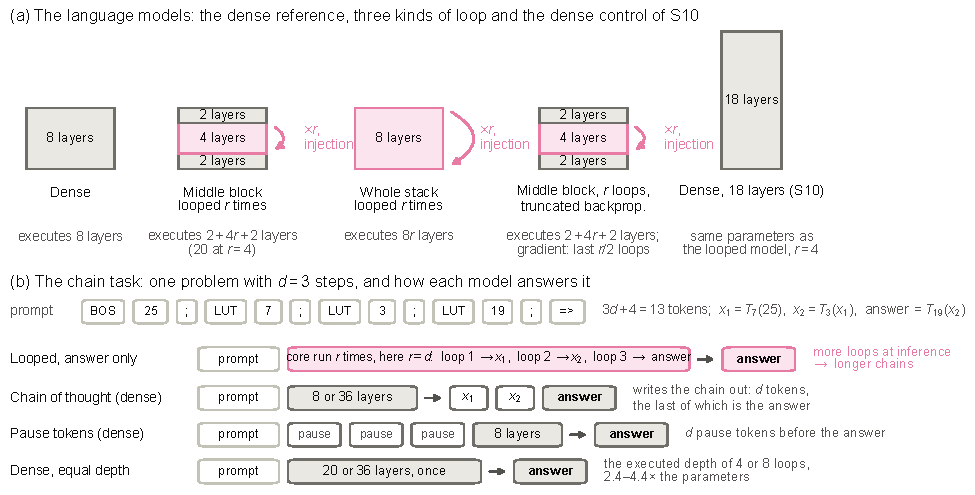
\includegraphics[width=\linewidth]{fig2_schematic}
  \caption{The models and the chain task. \textbf{(a)}~Every language model of the pre-registered grid has eight unique layers. A
  middle-block looped model runs its middle four layers $r$ times; a whole-stack model runs all eight. Each loop starts
  from a linear map of the previous state concatenated with the prelude output (input injection). With truncated
  backpropagation, only the last $r/2$ loops receive gradients. S10 adds dense models with 18 layers and about the looped model's number of parameters (Section~\ref{sec:depth}). \textbf{(b)}~A chain-task problem with $d = 3$ lookups in fixed
  random tables $T_k$ (\texttt{LUT k}: look up table $k$; BOS: the start marker). The looped model answers in one forward pass and computes the chain inside the loop (drawn with
  one loop per step); run for more loops, it solves longer chains. A dense chain-of-thought model writes the $d$ values
  of the chain, the last of which is the answer. A dense model with $d$ pause tokens and a dense model of the looped
  model's executed depth answer in one pass.}
  \label{fig:schematic}
\end{figure}

\subsection{Models}
\label{sec:models}

All language models of the grid (Figure~\ref{fig:schematic}a) are decoder-only transformers with eight unique layers of
width $w$. They use pre-norm RMSNorm, SwiGLU feed-forward blocks (hidden size $\tfrac{8}{3}w$), rotary position
embeddings, attention heads of dimension 64, no biases, untied input and output embeddings, a 16k BPE vocabulary trained
on the training data, and a context of 1024 tokens.

The models differ only in how they run these layers. A \emph{dense} model runs its eight layers once. A
\emph{middle-block} looped model runs the first two layers once (the prelude), the middle four $r$ times (the core, or
looped block) and the last two once (the coda), so it executes $2 + 4r + 2$ layers; a \emph{whole-stack} looped model
runs all eight layers $r$ times.


Each loop starts from a linear map of the previous state concatenated with the prelude output (for the whole stack,
which has no prelude, the embedded input). This input injection, as in Huginn \citep{geiping2025scaling}, has $2w^2$
parameters; the first state is zero. Every residual branch is scaled by $(L/12)^{-1/2}$, a depth rule in which $L = 8$ is the number of unique layers and 12
the reference depth, and by a further $1/r$ inside the core. The scaling is meant to keep the best learning rate
independent of $r$ \citep{wang2026residual}; Appendix~\ref{app:training} checks this. Backpropagation runs through all
loops or, in \emph{truncated} runs, through the last $r/2$ loops only. A model's \emph{executed depth} is the number of
layers it runs: 8 for the dense model and $2 + 4r + 2$ for the middle block. Most text results are for \emph{the 4-loop
model}: the middle block looped 4 times with full backpropagation, which runs 20 layers.

There are five sizes, named by their approximate non-embedding parameters: 10M, 20M, 40M, 80M and 160M, with widths 320
to 1280. Their parameter counts are $N = 15.4$M, 26.8M, 50.1M, 92.7M and 179.6M. $N$ counts the non-embedding parameters and
also the output head \citep{porian2024resolving}, which is large at small widths with a 16k vocabulary (Table~\ref{tab:sizes} in
Appendix~\ref{app:training}).

\subsection{Data, training and the grid}
\label{sec:grid}

Every run, except those of one supplementary experiment that varies the data order (S7), reads a prefix of one
fixed-order stream: files 000--012 of
FineWeb-Edu sample-10BT \citep{penedo2024fineweb}. The stream has 10.4B tokens with our tokeniser and the longest run uses
9.9B, so no run sees a document twice. The main validation set is 50M held-out FineWeb-Edu tokens from file 013. Three
further sets of 20M tokens come from SlimPajama \citep{soboleva2023slimpajama}, FineMath \citep{allal2025smollm2} and
GitHub code (Appendix~\ref{app:training}).

We use AdamW ($\beta = (0.9, 0.95)$, weight decay 0.1, gradient clipping 1.0) with one learning
rate per width, chosen by a sweep on the dense models and used unchanged for the looped models. This rate applies to the
embedding and output layers; the hidden layers use $(8/12)^{-1/2}$ times it, by the same depth rule as the residual
scaling (Appendix~\ref{app:training}). A budget is the number of training tokens per parameter, written $10N$ for ten tokens
per parameter. The schedule is warm-up--stable--decay with cooldown branches \citep{hagele2024scaling}: each run has
one constant-rate trunk, and for each budget a cooldown branches off it at 80\% of the budget and decays the rate
linearly to zero at the budget. Each run therefore gives one result per budget.

Looped runs have budgets of $10N$, $20N$ and $40N$; dense runs $5N$ to $80N$ ($40N$ at 160M). Each looped size
(10M--80M) has ten cells: the middle block with $r = 2$, 4 and 8 and full backpropagation, and with $r = 4$ and 8 and
truncated backpropagation; and the same five for the whole stack. Each size also has one dense model. Every looped cell and dense model has three seeds at
10M--40M and one at 80M, and a 160M dense model serves as a reference: 100 looped and 11 dense runs, 111 in the
pre-registered grid. Seeds change the initialisation,
not the data order.

Extensions of the grid, reported as exploratory, add a 160M 4-loop model and a second 160M dense seed, and continue
10M models to $160N$ and 20M models to $80N$
(Appendix~\ref{app:training} lists the cells and seeds). They also train 20M models with a random loop count, a
regime the pre-registration declared out of scope. Ten supplementary experiments, S1--S10, ran under plans frozen before their runs
(Table~\ref{tab:supp} in Appendix~\ref{app:training}). Everything ran on four RTX 4090 GPUs, about 19 days of wall-clock
time in all.

\subsection{Measurement}
\label{sec:measurement}

Losses are in nats per token on the main validation set. Across initialisation seeds, the loss of the 20M dense model
spans 0.014--0.024 nats at $10N$--$40N$ (0.004--0.008 at 10M and 40M; 0.003--0.07 across the looped cells at 20M).
Pairing runs by seed does not remove this noise. Runs with the same seed and width start from the same weights in the
layers they share and read the same data, yet the gap between the 4-loop model and the dense model of the same seed
varies across seeds by 0.005--0.020 nats at 10M, 0.032--0.045 at 20M and 0.003--0.005 at 40M. A difference of 0.01
nats in one seed is therefore within the noise at 10M--20M and resolvable at 40M. The grid's results at 10M--40M are
means over three seeds.

The pre-registered analysis measures the value of a loop through the effective size of a looped model, $\Neff = \Nonce + r^{\varphi}\Nrec$
\citep{schwethelm2026how}, where $\Nonce$ counts the parameters run once and $\Nrec$ those in the loop. Unlike
\citet{schwethelm2026how}, who count non-embedding parameters only, we include the output head in $\Nonce$, as in $N$.
A dense ``ruler'' $L(N, D) = E + A N^{-\alpha} + B D^{-\beta}$ is fitted to the dense runs
\citep{hoffmann2022training,besiroglu2024chinchilla} with a Huber loss in log space and block-bootstrap intervals
(Appendix~\ref{app:fits}). With the ruler fixed, the primary analysis fits one $\varphi$ for each loop type, that
is, each combination of looped block and backpropagation (the four rows of Table~\ref{tab:prereg}), so that the ruler
evaluated at $\Neff$ matches the looped losses. A joint fit of the ruler and all $\varphi$ is the pre-registered
secondary analysis.

Three further measures need no fitted law. The \emph{gap} is the looped minus the dense loss at equal parameters and
tokens, with the same seed. The \emph{dense size of equal loss}, $\Nstar$, is the size of a dense model that would reach the looped model's
  loss on the same number of training tokens. We read each measured dense size's loss at that token count and
  interpolate $\log N$ linearly in the loss. The \emph{multiplier} $M = \Nstar/N$ says how many dense parameters each
  parameter of the looped model is worth; $M > 1$ means the looped model beats a dense model of its own size. A local
  exponent $\varphi_{\mathrm{loc}}$ is defined by $\Nstar = \Nonce + r^{\varphi_{\mathrm{loc}}}\Nrec$. Finally, the
\emph{equal-compute gap} is the looped loss minus the loss of a dense model of the same size trained with the
  same FLOPs. We convert a looped run's training FLOPs (counted over executed layers, including attention and the output
  head) into the tokens a dense model of the same size could have seen with them. We then read the
  dense loss at that number of tokens off the measured dense curve. Where that point lies beyond the measured curve, two extrapolations bound it (Section~\ref{sec:equalcompute}).

\subsection{Hypotheses and evidence labels}
\label{sec:hypotheses}

The pre-registration was frozen on 2026-09-23, before any training run. It states four hypotheses with decision rules
(Appendix~\ref{app:prereg}):
\begin{itemize}
  \item \textbf{H1}: truncated backpropagation lowers $\varphi$, under both an equal-token and an equal-FLOP accounting.
  \item \textbf{H2}: a looped middle block has a higher $\varphi$ than a looped whole stack.
  \item \textbf{H3}: the gain from extra loops saturates in $r$, so that a geometric form
  $\Neff = \Nonce + \Nrec(1-\rho^r)/(1-\rho)$, with a fitted ratio $\rho$, extrapolates better than $r^{\varphi}$ to a
  held-out size.
  \item \textbf{H4}: the compute-optimal $r$ is small at matched training FLOPs and larger at matched deployment FLOPs.
\end{itemize}
Each result carries one of three labels. \lbl{Pre-registered} results test a hypothesis and decision rule frozen
before training. \lbl{Pre-specified} results were written into a plan frozen before the runs they describe: the
synthetic design (2026-10-09) and the three supplementary plans (2026-10-13, 2026-10-15 and 2026-10-27). These plans
call their experiments exploratory because they lie outside the pre-registration, but their quantities and readings were
fixed before the runs. \lbl{Exploratory} results were chosen after seeing data.
Every departure from a frozen document is dated in the deviation log.

\section{What a loop is worth on text}
\label{sec:text}

\subsection{The pre-registered law cannot say what a loop is worth}
\label{sec:verdicts}

The pre-registration measured the value of a loop by one number per loop type: the exponent $\varphi$ of
$\Neff = \Nonce + r^{\varphi}\Nrec$, read off a dense ruler fitted to the grid's 54 dense results (one result per run
and budget). Five model sizes were
too few for this. The ruler puts its irreducible loss at the lowest value the fit allowed ($E = 0.050$) and its parameter
exponent at $\alpha = 0.054$, far below the usual value of about 0.3, because five sizes cannot pin down $E$, $A$ and
$\alpha$ separately. $\varphi$ inherits this weakness: it is 0--0.17 per loop type with the primary fit, and 0--0.41 with the joint fit over all 352 results (two of the grid's results are excluded;
Appendix~\ref{app:prereg}), which gives $\alpha = 0.267$ (Table~\ref{tab:prereg}).

Under the pre-registered decision rules, none of the four hypotheses held as stated. Table~\ref{tab:prereg} gives the verdicts and
Appendix~\ref{app:prereg} the details. For example, truncated backpropagation was predicted to lower $\varphi$ (H1). With truncation, $\varphi$ was lower in the middle block, though the intervals
overlap, and higher in the whole stack, where truncation also lowered the loss of the whole stack looped 4 times at every size.
Truncated runs also had most of the loss spikes (Appendix~\ref{app:training}).

Fitted separately at each size against the same ruler, and allowed to be negative, $\varphi$ of the 4-loop model is
$-0.32$, 0.19, 0.39, 0.52 and 0.65 from 10M to 160M \lbl{(exploratory)}. These values come from the same weak ruler, so we use only their direction: the value of a
loop rises with model size, and a single $\varphi$ per loop type averages over very different regimes. The rest of this
section therefore measures the value of a loop without a fitted law.

\begin{table}[t]
  \centering
  \caption{Pre-registered results. Top: $\varphi$ per loop type on the main validation set (equal-token accounting, $N$
  including the output head), from the primary analysis with 95\% block-bootstrap intervals and from the secondary joint fit; both fits bound
  $\varphi$ below by 0. Bottom: the verdicts on the four hypotheses under the frozen decision rules (in full in
  Table~\ref{tab:verdicts}).}
  \label{tab:prereg}
  \footnotesize
  \begin{tabular}{lcc}
    \toprule
    Loop type & $\varphi$, primary [95\% interval] & $\varphi$, joint fit \\
    \midrule
    Middle block, full backpropagation & 0.13 [0.02, 0.27] & 0.41 \\
    Middle block, truncated            & 0.00 [0.00, 0.17] & 0.29 \\
    Whole stack, full backpropagation  & 0.00 [0.00, 0.16] & 0.00 \\
    Whole stack, truncated             & 0.17 [0.10, 0.20] & 0.29 \\
    \bottomrule
  \end{tabular}

  \vspace{0.5em}
  \begin{tabular}{>{\raggedright\arraybackslash}p{0.56\linewidth}>{\raggedright\arraybackslash}p{0.38\linewidth}}
    \toprule
    Hypothesis & Verdict \\
    \midrule
    H1: truncation lowers $\varphi$ & Not supported \\
    H2: a middle block has a higher $\varphi$ than the whole stack & Depends on the measure \\
    H3: the gain from loops saturates in $r$ & Not supported \\
    H4: the best $r$ is small at equal training compute, larger at equal deployment compute & First half trivially (dense is best); second not supported \\
    \bottomrule
  \end{tabular}
\end{table}

\subsection{Measured directly, a loop's value rises with model size and data}
\label{sec:multiplier}

\begin{figure}[t]
  \centering
  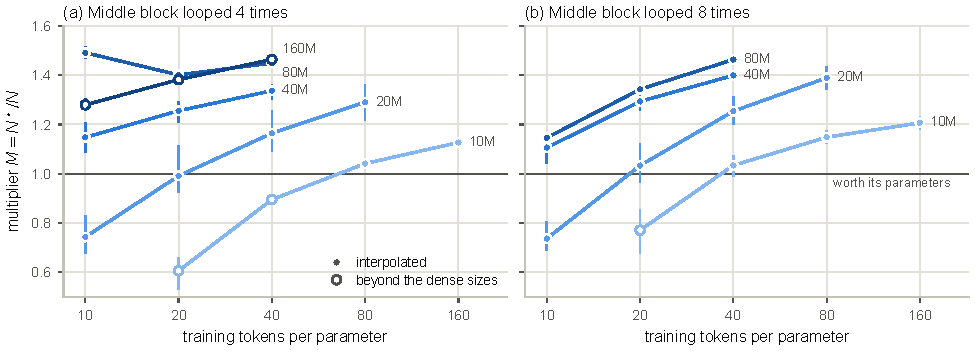
\includegraphics[width=\linewidth]{fig2_multiplier}
  \caption{What each parameter of a middle-block looped model is worth in dense parameters: the multiplier
  $M = \Nstar/N$. $\Nstar$ is the size of the dense model that reaches the same loss on the same number of training
  tokens, interpolated between the measured dense sizes (including the dense models trained longer in S4,
  Section~\ref{sec:equalcompute}). $M = 1$: as good as a dense model of its own size. Open markers: $\Nstar$ lies beyond
  the largest or smallest dense size, by at most a factor of two. Diamonds: dense models with 18 layers and about the
  looped model's number of parameters (Section~\ref{sec:depth}). Bars: 95\% intervals from resampling the seeds (three; two at
  160M; one at 80M), a rough guide with so few seeds.}
  \label{fig:multiplier}
\end{figure}

The dense runs themselves can serve as the ruler. For each looped model, we read the loss of every measured dense size
at the looped model's number of training tokens, and interpolate the dense size $\Nstar$ that has the same loss. The
multiplier $M = \Nstar/N$ is then what each parameter of the looped model is worth in dense parameters
(Figure~\ref{fig:multiplier}, \lbl{exploratory}).

For the 4-loop model, $M$ depends on size and data. At 10M--20M with 10--20 tokens per
parameter, $M$ is 0.6--1.0 where it can be read: the looped model is worth at most a dense model of its own size. At 40M--160M with 20--40 tokens per
parameter, $M$ is 1.26--1.46. For some of these values, $\Nstar$ lies outside the measured dense sizes, by less than a
factor of two: below the smallest for the 10M value of 0.6, and above the largest for the 160M values. At 10M with 10 tokens per parameter, $M$ is not reported: the looped model is worse than both dense models
measured at that number of tokens, and these two are out of order (the 20M one, trained on 5.7 tokens per parameter,
is worse than the 10M one), so the dense size of equal loss cannot be extrapolated (Appendix~\ref{app:fits}).

$M$ rises with data at 10M--40M and at 160M. At 80M, with one seed, it is flat:
1.49, 1.40 and 1.45 at $10N$, $20N$ and $40N$. Fitting $\log_2 M$ as a plane in $\log_2 N$ and $\log_2$(tokens per parameter) gives a factor of 1.21 per
doubling of model size and 1.14 per doubling of tokens per parameter (Appendix~\ref{app:fits}). Looping 8 times
instead of 4 raises $M$ by up to 0.16 at 10M--20M (0.11 among the values within the measured dense sizes), with no
consistent change from 40M on.

$M$ counts all of $N$, including the output head, which lies outside the looped block (34\% of $N$ at 10M, 21\% at
40M). The local exponent $\varphi_{\mathrm{loc}}$ credits the whole gain to the looped parameters; it is negative where
$M < 1$ ($-0.84$ at 20M with 10 tokens per parameter) and 0.22--0.55 from 40M on. If $N$ excludes the head, as in
\citet{schwethelm2026how}, $\varphi_{\mathrm{loc}}$ is 0.32--0.50 at 40M--160M with 20--40 tokens per parameter, close
to their $\varphi = 0.46$ (Appendix~\ref{app:fits}).

The shared learning rate does not create this trend. A supplementary experiment (S1, \lbl{pre-specified};
Appendix~\ref{app:lr}) re-tuned the learning rates of the dense model and the 4-loop model at 10M--40M, with one seed
(two at 20M). Re-tuning changed the gap between them by at most 0.005 nats at 20M--40M. At 10M, where the looped
model preferred lower rates, it improved the looped model's standing by about 0.02 nats. With each model at its best
rate, the size trend at $40N$ is somewhat smaller but meets the plan's criterion, which asks that it keep more than half of its value at the shared rate. The data trend at 10M is larger than at the shared rate: the gap goes from $+0.082$ at $10N$ to $-0.059$ at
$160N$.

Converted to $M$, the equal-parameter results of Parcae \citep{prairie2026parcae} and Ouro \citep{zhu2025scaling}
reach a similar level (1.23--1.46 at 134M--770M), but not the same trend: Parcae's values fall with size at about 80
tokens per parameter, and Ouro's rise with size while its tokens per parameter fall. The shallower looped blocks of
\citet{saunshi2025reasoning}, trained on about 750--1500 tokens per parameter, reach 1.47--1.95
(Appendix~\ref{app:published}). The published results barely sample models below 40M trained on 20 or fewer tokens per parameter, where we find the looped model worth at most a dense model of its own size. A value that rises with tokens per parameter is not captured by effective-parameter laws in which the factor applied to
the looped parameters does not depend on the training tokens \citep{schwethelm2026how,chen2026moe}.

Every dense model of this ruler has eight layers, while the 4-loop model executes 20. At a fixed size, deeper and thinner
models do better below a billion parameters \citep{liu2024mobilellm}, though the shape matters little over a wide range
of shapes \citep{kaplan2020scaling}. So $M$ may measure what depth gives at a fixed size rather than what sharing gives.

\subsection{At 40M, a deeper dense model of the same size recovers about half of the loop's advantage}
\label{sec:depth}

To separate depth from sharing, a supplementary experiment (S10, \lbl{pre-specified}) trained dense models with 18 layers and about the looped model's number of parameters: 18 layers of
width 320 ($N = 28.1$M) at 20M and of width 448 ($N = 51.2$M) at 40M. Their executed depth of 18 is close to the 4-loop model's 20. They use the grid's recipe, data, budgets and three
seeds. Their learning rate follows the grid's rule
(Section~\ref{sec:grid}): the embedding and output layers use the rate of their width, and the hidden layers use
$(18/12)^{-1/2}$ times it. We call this the
rule's rate. Their multiplier $M_{\mathrm{deep}}$ is read off the same 8-layer dense runs and compared with the 4-loop model's
multiplier $M_{\mathrm{loop}}$ at the same size and budget. The plan fixed in advance how to interpret them. It defines
$R = \log M_{\mathrm{deep}} / \log M_{\mathrm{loop}}$, computed at 40M for each budget and averaged over the three
budgets, as the share of the looped model's advantage that a dense model of the same size and nearly the same
depth recovers. The plan reads $R \geq 0.75$ as ``most of the advantage is a depth effect'', $0.25 \leq R < 0.75$ as ``partly depth, partly sharing'' and $R < 0.25$ as ``looping buys more than depth''.

At 40M, the deep dense model is worth 1.10, 1.11 and 1.11 dense parameters
per parameter at $10N$, $20N$ and $40N$; the looped model is worth 1.15, 1.26 and 1.34 (Figure~\ref{fig:multiplier}a,
diamonds). So $R$ is 0.50 (0.41--0.62 when the three seeds are resampled), in the band the plan reads as ``partly depth, partly sharing'', as it predicted. At 40M, the value of depth does not grow with data, but the looped model's lead
over the deep model does. The lead is 0.003 nats at $10N$, 0.015 at $20N$ and 0.029 at $40N$, with the same sign in all three seeds
at the two longer budgets. At 20M, the deep model is narrow (width 320) and worse than the 8-layer model of the same size
($M_{\mathrm{deep}} = 0.84$--0.94). There, depth explains none of the looped model's advantage at $40N$
($M_{\mathrm{loop}} = 1.16$; the plan reports 20M descriptively).

The deep model's learning rate was
checked with one seed (seed 42). At 40M its best rate was the highest one tried, 1.41 times the rule's rate, at all three budgets, beating the rule's rate by 0.014, 0.006 and 0.001 nats at $10N$, $20N$ and $40N$. Because it beat the rule's rate by more than 0.01 nats at $10N$, the plan asks for a second
computation with each model at its best tested rate (Appendix~\ref{app:s10}). Computed that way, the deep model is ahead of the looped one
at $10N$ by 0.010 nats ($M = 1.37$ against 1.18, so $R = 1.91$), and $R$ is 0.56 and 0.34 at $20N$ and $40N$ (0.45 and
0.37 for the same seed at the rule's rate). These readings may understate the deep model, because its
best rate lies at the edge of the range tried and the plan had no rule to extend the range. Their average, 0.94, would count as ``most of the advantage is a depth effect''. But this average is dominated by the $10N$ value, where $\log M_{\mathrm{loop}}$ is only 0.17 and the ratio is
unstable, and the plan keeps the value at the rule's rate as the primary result. The deep model also costs about half the training compute of the
looped model: 406M against 835M FLOPs per token at 40M.

About half of the looped model's advantage at equal parameters at 40M thus comes from depth. With each model at its best tested learning rate, depth accounts for all of it at the shortest budget, in the one seed
tried:
the deep model's lead there, 0.010 nats, is twice the range of this gap across the three seeds at the rule's rate
(Table~\ref{tab:s10}). At 20M depth explains none of the advantage, and at neither size does depth recover the
part that grows with data (Appendix~\ref{app:s10}).

\subsection{At equal training compute, the dense model wins all but one measured comparison}
\label{sec:equalcompute}

At equal parameters, a middle block looped 2, 4 or 8 times costs 1.4--1.5, 2.2--2.4 or 3.7--4.1 times the training FLOPs
per token of the dense model. For an equal-compute comparison, we give the dense model the tokens it could have seen
with the looped run's compute, and read its loss off the measured dense curve \lbl{(exploratory)}.

\begin{figure}[t]
  \centering
  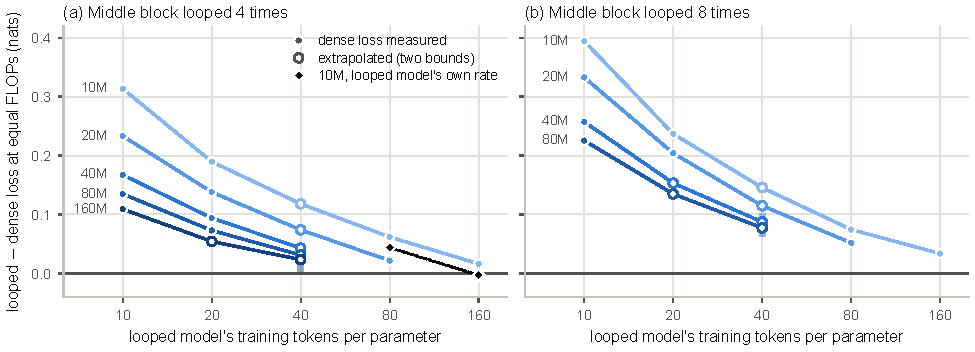
\includegraphics[width=\linewidth]{fig3_equal_compute}
  \caption{Equal training compute: looped minus dense loss, when the dense model of the same size is trained on the
  tokens that the looped run's compute would buy (positive: dense better). Filled markers: the dense loss is measured,
  including the dense models trained longer in S4, to $640N$ (10M) and $320N$ (20M). Open markers with bars: the dense loss is
  extrapolated, and the bar spans the two extrapolations (from the power law to the extended last segment). Diamonds: the 10M model looped 4 times,
  trained at 0.35 times the dense rate, the lowest rate S1 tried (mean of two seeds; bars: seed range).}
  \label{fig:equalcompute}
\end{figure}

The grid and its extensions have 320 looped results. For 221 of them, the original dense runs reach the equal-compute
point, and at the shared learning rate the dense model won all of them, by at least 0.016 nats. Continuing the 10M dense models to $640N$ and the 20M ones to $320N$ (S4, \lbl{pre-specified})
turned 37 more comparisons into measured ones (Figure~\ref{fig:equalcompute}), and the dense model won these as well:
all 258 measured comparisons at the shared rate. These comparisons share dense curves, trunks and seeds, so they are not
independent.

The dense model's lead shrinks with data: for the 10M 4-loop model trained on $40N$, $80N$ and $160N$, it is $+0.119$ nats (with the dense loss extrapolated for one seed), $+0.062$ and $+0.016$. Table~\ref{tab:equalcompute} in Appendix~\ref{app:lr} lists the comparisons at the
largest budgets.

The remaining comparisons need an extrapolated dense loss, which two extrapolations bound: a power law fitted to
each dense curve, which favours looping, and an extension of the curve's last measured segment, which favours the dense model (Appendix~\ref{app:lr}). Of the 99 such comparisons before S4, looping came out ahead in 6 under the
power law, by at most 0.021 nats, all at the largest data per parameter. Where S4 measured such comparisons, the measured gaps fall about
halfway between the two extrapolations; 62 comparisons remain extrapolated.

With each model at its best tested learning rate (S1),
the dense model won 10 of the 11 comparisons (one of them, 40M at $40N$, on an extrapolated dense loss). The eleventh is
at 10M and $160N$, with the looped model at 0.35 times the dense rate. That was the lowest rate tried, and the looped
model's loss was still falling as the rate went down. There the two are level on average ($-0.011$ and $+0.005$ in two
seeds). It is the only measured equal-compute comparison in this study that the dense model does not win.

The deep dense models of Section~\ref{sec:depth} cost about half the looped model's compute per token, and they are ahead by 0.11--0.19 nats wherever their measured curves reach the equal-compute point \lbl{(exploratory)}.

\subsection{At deployment, the loop saves some weight memory but costs decoding time and KV cache for every executed
layer}
\label{sec:cost}

We measured inference on one RTX 4090 in bf16, with KV-cached decoding and a separate cache for every executed layer, so that decoding computes what the models
computed in training (S3, \lbl{pre-specified}; Appendix~\ref{app:cost}). At these sizes, decoding time follows
the number of executed layers. At equal parameters, a middle block looped 2, 4 or 8 times takes 1.5, 2.4--2.6 or
4.5--4.6 times the decoding time per token of the dense model, close to the ratios of executed layers.

At equal quality, the comparison is with the dense model that reaches the same loss when both are trained on 40
tokens per parameter, interpolated between the measured dense sizes. This differs from $\Nstar$, which holds the number
of training tokens fixed. Against it, the 4-loop
model needs less weight memory: 4\% less at 20M, rising to 19\% at 160M, where the dense model of equal loss is
extrapolated. But it needs 2.20--2.41 times the KV cache per token, 2.37--2.47 times the decoding time and about 1.6
times the peak memory at batch 32.

One way to cut this cost is to share the KV cache across loops. Each core layer then keeps one cache for all loops,
and every loop reads the earlier tokens' keys and values as they were written at those tokens' last loop. This would
remove most of the cache and memory cost, though not the decoding time. A supplementary experiment (S6, \lbl{pre-specified}) applied it after
training to 20M models of one seed, at the constant-rate checkpoint at $32N$ from which the $40N$ cooldown branches
off. The models include a 4-loop model trained at half the dense rate in S1. The comparison with the dense model at
the same checkpoint and on the same tokens was added after a review and is \lbl{exploratory}
(Appendix~\ref{app:deviations}). For every model that gains
from its loops, sharing costs 2.2 to 7.4 times that gain (0.09--0.17 nats, against gains of 0.019--0.046 over the dense
model), so each would end up worse than the dense model of its size. These gains come from one seed, and at 20M the
gap between a looped and a dense model varies across seeds by 0.032--0.045 nats (Section~\ref{sec:measurement}), so
the ratios are rough. By the S6 plan's thresholds (an increase above 0.02 nats ``degrades'', above 0.1
``breaks''), sharing degrades the 8-loop model (by
0.09 nats) and breaks the truncated 8-loop model (0.14), the 4-loop model (0.17) and, at the boundary, the 4-loop
model at half the rate (0.10; Appendix~\ref{app:cost}). Sharing costs nothing only for the models trained with a random loop count, whose block
contracts to a fixed point (Section~\ref{sec:mechanism}); these models gain nothing over the dense model. We tested neither of two routes that may avoid this cost: training the loop to converge, and
training with a shared cache from the start. \citet{monea2026shared} pretrain looped models with a scheme in which only the first loop
writes the cache, and find that it costs no quality in their setting.

\paragraph{What the loop buys on text.} Where the loop helps at equal parameters, it saves parameters and data but costs compute. From about 40M to 160M,
with 20--40 tokens per parameter, each parameter of the 4-loop model is worth about 1.3--1.5 dense parameters, more with more data at most sizes. At 40M, a dense model of the same size and nearly the same depth gets about half of that advantage for half the
compute (all of it at the shortest budget once its learning rate is tuned, in one seed), but not the part that grows
with data. At equal training compute the dense model wins every measured
comparison but one, and at deployment the loop costs decoding time and KV cache for every executed layer. The next two sections test the second
claim: that running more loops at inference solves harder problems.

\section{On text, extra loops at inference never help}
\label{sec:mechanism}

If the loop iterated towards an answer, the state after each loop would carry a better prediction than the state
before it, and running more loops at inference would help. At these sizes, it does not. To see what the loop computes
instead, we probed trained models loop by loop, on trunk checkpoints at $32N$ before cooldown \lbl{(exploratory)}. We
read the state after each loop with the model's own output layers (the coda and the output head), with a learned
linear map placed before them, and with a learned linear head in their place (Appendix~\ref{app:fits}). Reading it
through the model's own output layers, a logit lens, is the same as running the model with that many loops; the learned
map is a tuned lens trained on the next token. Figure~\ref{fig:mechanism} shows three training regimes.

\begin{figure}[t]
  \centering
  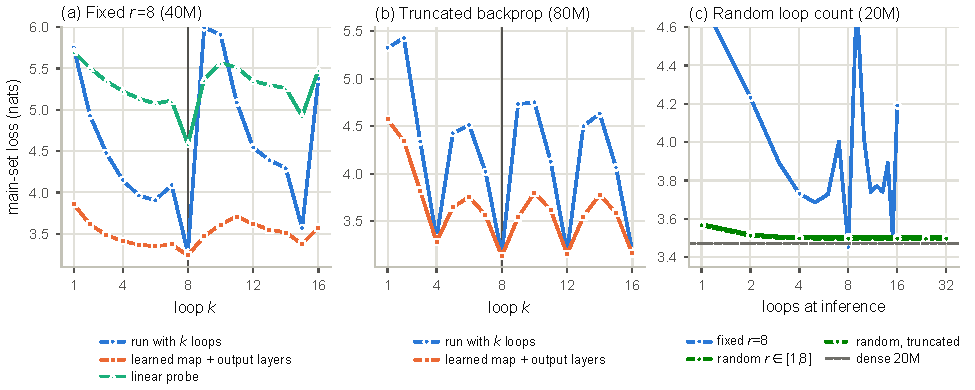
\includegraphics[width=\linewidth]{fig4_text_mechanism}
  \caption{What the looped block computes on text (main-set loss of trunk checkpoints at $32N$; values above the top of
  a panel are clipped). \textbf{(a)}~Fixed loop count: a 40M middle block trained with 8 loops (mean of three seeds),
  read after each loop $k$ by running the model with $k$ loops, by a learned linear map placed before the output layers,
  and by a learned linear head in their place. The model reaches its low loss only at its training loop count. \textbf{(b)}~Truncated backpropagation (80M
  whole stack, $r = 8$, gradients through the last 4 loops): the state returns to almost the same point every four loops.
  \textbf{(c)}~Trained with a random loop count (20M middle block, $r$ drawn from 1--8 at every training step), the block
  contracts to a fixed point: the loss is flat from about four loops on and no better than the dense model, with or
  without truncation.}
  \label{fig:mechanism}
\end{figure}

Trained with a fixed count of 8 loops, the middle block behaves like a fixed-length program. The model reaches its low
loss only at 8 loops, and running it with fewer or more loops makes the loss much higher (Figure~\ref{fig:mechanism}a).
Read with a learned map, the state after loop 4 is already within 0.1--0.2 nats of the final loss, and loops 5--7 add
little. The last loop is a large non-linear move that rewrites the state into what the output layers expect: for
37--47\% of the tokens, the predicted token changes for the last time at loop 8. These patterns held in all three seeds
at 20M and 40M, and in the one seed at 80M.

With truncated backpropagation, the whole stack learns a periodic cycle. When it is trained with 8 loops and gradients
through only the last four, its state returns to almost the same point every four loops (Figure~\ref{fig:mechanism}b).
The model works at 4, 8, 12 or 16 loops and gains nothing from more loops. The same minima at 4, 8 and 12
loops appear at 20M and in both probed 40M seeds. We did not probe a middle block trained with truncated backpropagation.

Drawing the loop count from 1--8 at every training step, as Huginn does with a different distribution
\citep{geiping2025scaling}, gives a block that contracts to a fixed point. Its loss is flat from about four loops to 32
(Figure~\ref{fig:mechanism}c; one seed at 20M, with full and with truncated backpropagation). Such a model is robust to
the loop count, but at 8 loops, the top of its training range, it is 0.05 nats worse than the model trained with a
fixed 8 loops and no better than the dense model. Parcae's models, trained with a sampled loop count at 140M--770M, keep
an advantage, so our result, from one seed at one size, may be specific to small models or to our distribution.

Lower learning rates give flatter curves over the inference loop count. In S1, whose plan lists this as an exploratory
question (Q5), the loss of the 4-loop model at 10M, 20M and 40M varies by 0.36--0.77 nats over 4--16 loops at 0.5 times
the dense rate, and by 3.4--4.6 nats at 1.41 times. At every rate, though, the better of 8 and 16 loops was worse than
the training count of 4.

The looped model's gain over the dense model on web text is small and spread across tokens \lbl{(exploratory)}. About
half of the tokens improve, and the gain is no more concentrated on hard tokens than the difference between two dense
seeds is. On math and code text the gains are larger, but there the spread between seeds is 10--100 times larger as
well, and the code set is more sensitive to the data order than to the initialisation (S7, \lbl{pre-specified};
Appendix~\ref{app:fits}). We draw no conclusions from differences on those sets.

On web text at these sizes, then, the loop gains little from iterating, and running it for more loops than it was
trained with never helped.

\section{On a serial task, a loop buys extendable depth}
\label{sec:serial}

To test the second claim where iterating should matter, we built the chain task, a task that needs serial steps, and
froze its design, conditions and predictions before its main runs; it uses the same architecture as the language
models. Pilot runs then led to three changes before any formal run, all to make the task
learnable: the operations became lookup tables instead of modular arithmetic, a curriculum was added, and training was
lengthened. The last of these came after a one-seed pilot of all conditions, and the
learning-rate protocol was fixed after that (Appendix~\ref{app:deviations}).

\subsection{The task and the conditions}
\label{sec:task}

A problem lists a start value and a sequence of table lookups (Figure~\ref{fig:schematic}b), for example
\texttt{25 ; LUT 7 ; LUT 3 ; LUT 19 ; \ldots\ =>} after a start marker. Here \texttt{LUT k} means ``look up the
current value in table $T_k$'', one of 32 fixed random tables that map $\{0,\ldots,96\}$ to itself. Each lookup is one
step: the $j$-th gives the intermediate value $x_j$, and a chain of $d$ steps has $d$ lookups and a prompt of $3d + 4$
tokens. The model must output the final value in a single forward pass, and the loss is taken at the answer position
only. Two consecutive lookups can form any of the $32 \times 32 = 1024$ compositions of two tables, so a model that
skips steps must memorise tables of compositions, which grow rapidly with the number of steps skipped. Because
composition is associative, the chain could in principle be computed in fewer serial steps than it has lookups
\citep{liu2022shortcuts}.

Models are trained on chains of 1--8 steps for 32{,}000 training steps, with batches of 512 problems sampled online and
a curriculum that widens the range of lengths over the first half of training. They are tested on 2{,}000 newly drawn
problems at every length from 1 to 24. Chains longer than 8 steps never occur in training, but short ones repeat: every
test problem with 1 or 2 steps, and about half of those with 3, also occurs in training (there are only 3{,}104
one-step problems).

All models have width 256. The dense models have 8, 20 or 36 layers (6.5M, 16.1M and 29.0M parameters); those with 20
and 36 layers match the executed depth of the looped models with 4 and 8 loops. The looped models have 8 layers (6.6M
parameters), with a middle block of four layers looped $r$ times. They are trained with $r = 2$, 4 or 8 loops, with a
random loop count drawn from 1--8 at every training step, or with as many loops as the chain has steps (``loops =
steps'', the regime of \citealp{fan2025looped}). A fourth regime, loops = steps with a few random extra loops (S9), is
introduced in Section~\ref{sec:stopping}. In S5 (\lbl{pre-specified}), dense models write the values of the chain out
as tokens, the last of them the answer. This chain of thought \citep{wei2022chain} is trained from scratch on the
written values, as in scratchpad training \citep{nye2021show}, with 8 layers (the looped models' size) and with 36 (the
8-loop model's executed depth). We also train an 8-layer dense model given $d$ pause tokens before the answer
\citep{goyal2024think}.

Every condition has five seeds, and its learning rate was chosen by a sweep on in-range accuracy only. The looped
models' rates came out 4--8 times lower than that of the 8-layer dense model, which has the same unique layers
(Appendix~\ref{app:synthetic}). The design fixed five predictions (P1--P5, Section~\ref{sec:predictions}). A planned
control task, pointer chasing, was not learned by any condition tried on it and was dropped
(Appendix~\ref{app:synthetic}).

\subsection{Within the training range, a loop adds depth, and a written chain of thought does so more cheaply}
\label{sec:inrange}

At equal parameters, the largest solvable length rises with the number of loops: from 4.2 steps for the 8-layer dense
model to 6.4, 8.0 and 9.0 steps with 2, 4 and 8 loops (seed means; Table~\ref{tab:chain}, \lbl{pre-specified}). Within
the training range, the 8-loop model is at 0.998 where the 8-layer dense model is at 0.62.

\begin{table}[t]
  \centering
  \caption{The chain task, trained on 1--8 steps (seed means; chance is 0.01; accuracies rounded, and only the
  chain-of-thought models are exactly perfect in range). \emph{Largest solvable length}: the longest chain length up to
  which every length is solved with accuracy $\geq 0.9$ (mean, and min--max over five seeds). The frozen design's measure, the largest length solved at $\geq 0.9$ without requiring every shorter length, gives the
  same values in the \emph{Training loops} column and differs only for 2 loops under \emph{More loops} (10.4 instead of
  8.6). \emph{Training loops}: at the training loop count (8 for the random loop count, $d$ for loops = steps; dense
  models as trained). \emph{More loops}: the training loop count or any larger count tried, including $d$ loops,
  whichever is best for each seed, chosen using the test answers (a reference, not a rule a model could apply); the set
  of counts was widened after the results (Appendix~\ref{app:deviations}). ``---'': not applicable. \emph{Layer passes}:
  executed layers times tokens processed for a 12-step problem, that is, a prompt of 40 tokens, plus the 11 written values that precede the answer for the
  chain-of-thought models (each fed back with a KV cache; the answer itself is not processed) or 12 pause tokens.}
  \label{tab:chain}
  \footnotesize
  \setlength{\tabcolsep}{2.6pt}
  \begin{tabular}{lccccccc}
    \toprule
    & & & Within the range & \multicolumn{2}{c}{Largest solvable length} & \multicolumn{2}{c}{Beyond the range} \\
    \cmidrule(lr){4-4}\cmidrule(lr){5-6}\cmidrule(lr){7-8}
    & & Layer & Acc. & Training & More & Acc.\ 12 steps & Acc.\ 16 steps \\
    Model & Params & passes & 1--8 steps & loops & loops & train.\ / more & train.\ / more \\
    \midrule
    \multicolumn{8}{l}{\emph{Equal parameters}} \\
    Dense, 8 layers               & 6.5M & 320  & 0.621 & 4.2 (4--5)   & ---           & 0.06        & 0.05        \\
    Looped, $r=2$                 & 6.6M & 480  & 0.906 & 6.4 (6--7)   & 8.6 (6--11)   & 0.05 / 0.64 & 0.04 / 0.33 \\
    Looped, $r=4$                 & 6.6M & 800  & 1.000 & 8.0 (8--8)   & 11.8 (10--15) & 0.03 / 0.83 & 0.03 / 0.28 \\
    Looped, $r=8$                 & 6.6M & 1440 & 0.998 & 9.0 (9--9)   & 11.2 (11--12) & 0.04 / 0.86 & 0.03 / 0.37 \\
    Looped, random loop count     & 6.6M & 1440 & 0.999 & 11.4 (10--13) & 12.2 (10--15) & 0.77 / 0.83 & 0.08 / 0.49 \\
    Looped, loops = steps         & 6.6M & 2080 & 1.000 & 12.8 (11--16) & 12.8 (11--16) & 0.96 / 0.96 & 0.37 / 0.37 \\
    Loops = steps + 0--4 extra (S9) & 6.6M & 2080 & 0.999 & 11.6 (11--12) & 12.2 (12--13) & 0.90 / 0.94 & 0.31 / 0.48 \\
    \midrule
    \multicolumn{8}{l}{\emph{Equal executed depth, which here is equal compute}} \\
    Dense, 20 layers (as $r=4$)   & 16.1M & 800  & 0.910 & 6.4 (6--7)  & ---           & 0.04        & 0.03        \\
    Dense, 36 layers (as $r=8$)   & 29.0M & 1440 & 0.999 & 8.0 (8--8)  & ---           & 0.02        & 0.02        \\
    \midrule
    \multicolumn{8}{l}{\emph{Dense models with written-out reasoning or pause tokens (S5)}} \\
    Chain of thought, 8 layers   & 6.5M  & 408  & 1.000 & 8.0 (8--8) & ---          & 0.01        & 0.01        \\
    Chain of thought, 36 layers  & 29.0M & 1836 & 1.000 & 8.0 (8--8) & ---          & 0.02        & 0.01        \\
    $d$ pause tokens, 8 layers   & 6.5M  & 416  & 0.566 & 4.0 (4--4) & ---          & 0.01        & 0.01        \\
    \bottomrule
  \end{tabular}
\end{table}

At equal executed depth, and so at equal compute, the looped models are at least as good as the dense ones. A dense
model of equal executed depth has the same width as the looped model and is trained for the same number of training
steps on the same problems. On this task it therefore costs about the same training and inference compute, but it has
2.4--4.4 times the parameters, and if the extra parameters matter, they help the dense model. The 20-layer dense model
solves 6.4 steps against 8.0 for 4 loops, though it did not fully learn the training range (0.91). Its learning rate
was chosen in a sweep whose runs were half as long as the formal runs, and in that sweep it reached 0.98
(Appendix~\ref{app:synthetic}). The 36-layer dense model solves 8.0 steps against 9.0 for 8 loops, and the two are
level within the range. These lengths are the plan's measure, the solvable length at the training loop count;
Section~\ref{sec:extension} discusses the \emph{More loops} columns.

On text, the dense model of equal compute has the looped model's size and more data. Here it has more parameters and
the same data, and it does not beat the loop. We do not take these two comparisons as evidence that the loop saves
compute, since one dense model did not fully learn the range and the other is level with the loop within it.

A written chain of thought is perfect within the training range and costs less than the loop. It scores 1.000 in every
seed and at every learning rate tried, where the 8-layer model that answers directly solves 4 steps. At any length it
needs under a third of the inference compute of the 8-loop model: 408 against 1440 layer passes at 12 steps
(Table~\ref{tab:chain}). The comparison favours it, because it is trained with a loss on every intermediate value and
the other models on the answer only. The plan stated this difference in advance, and a looped model with intermediate
supervision was outside it. Pause tokens add nothing: the pause model solves the same 4 steps as the model without
them.

\begin{figure}[t]
  \centering
  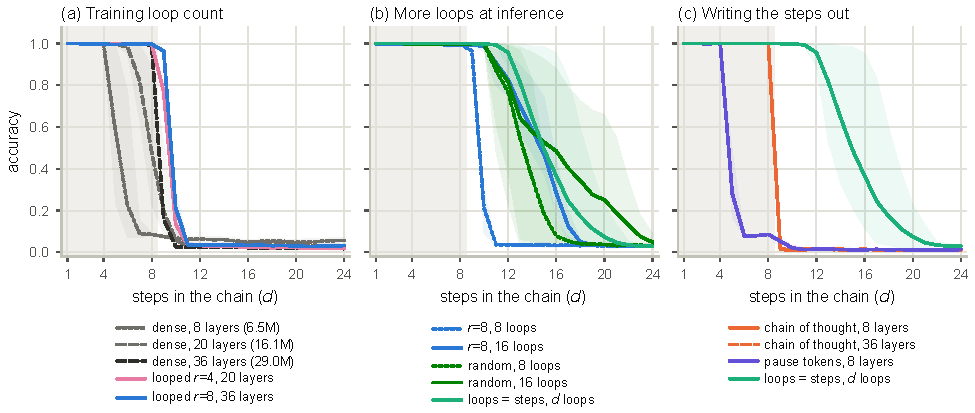
\includegraphics[width=\linewidth]{fig5_chain}
  \caption{The chain task, trained on 1--8 steps (shaded): accuracy against chain length, mean over five seeds (band:
  range). \textbf{(a)}~At the training loop count, looped models solve at least as far as dense models of the same
  executed depth, and none gets more than one step past the training range. \textbf{(b)}~With more loops at inference,
  the looped models solve longer chains; the model trained with as many loops as steps, run with $d$ loops, solves the
  longest chains at accuracy 0.9. \textbf{(c)}~Dense models that write the chain out are perfect within the training
  range and near chance beyond it; pause tokens add nothing (the loops = steps model is replotted for comparison).}
  \label{fig:chain}
\end{figure}

\subsection{Beyond the training range, only the loop extends}
\label{sec:extension}

We say that a model \emph{extends} if, given more computation at inference, it solves chains longer than those it was
trained on. At their training loop count, neither the dense models nor the fixed-loop models get more than one step
past the training range: at 12 steps, the dense models that answer directly score 0.01--0.06 and the fixed-loop models
0.03--0.05 (Figure~\ref{fig:chain}a).

Run with more loops, the looped models extend (Figure~\ref{fig:chain}b). The model trained with 8 loops solves 9 steps
at 8 loops and about 11 with 16 or 32. At 12 steps its accuracy rises from 0.04 to 0.83 at 16 loops, and to 0.86 when
the best loop count between 12 and 32 is chosen for each seed using the answers (seed means). The gain is limited,
though: at 16 steps the best is 0.37, with a wide spread across seeds. The model trained with a random loop count gains
as well (0.08 to 0.49 at 16 steps), against the frozen prediction that it would not. Run with as many loops as the
chain has steps, the loops = steps model solves the longest chains at accuracy 0.9 (12.8 steps). Part of this comes
from being told how long to run, since its loop count is the number of steps, which the prompt shows. With $d$ loops it
is 0.34--0.95 more accurate than with 8 at every length from 10 to 16 (we count from 10 steps, a choice made after the
results; at 9 steps the difference is 0.03).

The written chain of thought, perfect within the training range (Section~\ref{sec:inrange}), does not extend at all.
It scores 0.014 at 12 steps with 8 layers and 0.017 with 36, near the chance level of 0.010, on prompts on which the
looped models trained with 4 or more loops reach 0.83--0.96 (Figure~\ref{fig:chain}c). S5 had predicted at least 0.7
for the 8-layer model and at least 0.8 for the 36-layer one. The 8-layer model breaks at the start. On problems with
more than 8 steps, its first wrong token is one of the first three written ones in 97--98\% of the problems
\lbl{(exploratory)}, so its errors do not build up along the chain. Because the prompt of this task grows with the
number of steps, the chain of thought may be failing to generalise to longer inputs, a known weakness of transformers
\citep{zhou2024transformers,cho2024position}, rather than to more steps. The comparison cannot say whether a written
chain would extend on a task whose input length does not grow; we did not run such a task, and remedies for length
generalisation were outside the plan. Pause tokens do not extend either, as S5 predicted.

\subsection{The loop computes the chain step by step}
\label{sec:probes}

For each intermediate value $x_j$, we trained a linear probe on the state after every loop, on problems with 8 steps
and with the looped models running 16 loops (Figure~\ref{fig:probes}). The probes were planned in the frozen design;
the summaries below are \lbl{exploratory}. Each probe reads three prompt positions around step $j$ (its table number,
the separator after it and the next lookup token), and the best of the three counts.

With a loop for every step, the chain advances one step per loop. In the model trained with 8 loops, $x_j$ first
becomes decodable (probe accuracy $\geq 0.5$) at about loop $j$, at 1.0--1.1 loops per step in all five seeds. It
stays decodable afterwards, with a lowest probe accuracy at later loops of 0.96, averaged over the values. The loops =
steps model also computes one step per loop and keeps its values for its $d$ loops (lowest later accuracy 0.92), but
it loses them when run longer. It was never trained to keep looping after the last step, which is why it needs exactly
$d$ loops.

Models with fewer loops than steps pack several steps into each loop, about 1.6 with 4 loops and 2.4 with 2, in the
direction that \citet{zhang2026recurrence} predict. In these models the last values become decodable at the step
positions only after the training loop count: at loop 5 with 4 loops, and at loops 3--4 with 2.

The dense models compute the values late, from about layer 21 of 36, and in 5 of the 10 dense seeds (five at 20 layers
and five at 36) no intermediate value after $x_1$ is decodable. These probes are consistent with the extension results:
a loop that applies the same step each time can be run for more steps, while a stack that computes the chain in its
last layers cannot. A probe shows where a value can be read out; it does not show that the model uses the value.

\begin{figure}[t]
  \centering
  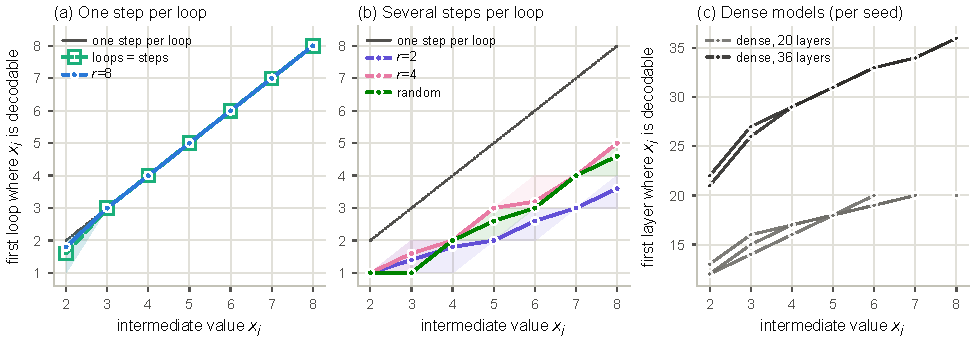
\includegraphics[width=\linewidth]{fig6_chain_probes}
  \caption{Where the intermediate values appear (probes on 8-step problems; a value counts as decodable at probe
  accuracy $\geq 0.5$). \textbf{(a)}~With a loop for every step, the chain advances one step per loop. \textbf{(b)}~With
  fewer loops than steps, each loop advances several steps (mean over seeds; band: range; looped models probed while
  running 16 loops). \textbf{(c)}~Dense models compute the values late in their depth (one line per seed). A seed in
  which only $x_1$, not plotted, and the answer are decodable appears as a single point at the last layer; the 20-layer
  seed with no decodable intermediate value is not shown.}
  \label{fig:probes}
\end{figure}

\subsection{The learning rate decides whether the loop learns the task within 32{,}000 training steps}
\label{sec:lrsynthetic}

At $10^{-3}$, a good rate for the dense models, the 8-loop model of the learning-rate sweep worked only at its training
count of 8 loops and at no other count from 2 to 32, like the language models of Section~\ref{sec:mechanism}. No
intermediate value became decodable one loop per step. But it had also learned the training range much worse: 0.54,
against 0.999 at $2.5\times10^{-4}$.

A supplementary experiment (S2, \lbl{pre-specified}) asked whether a high rate changes what the looped model learns or
how fast it learns. It trained the four looped conditions named in its plan ($r = 4$, $r = 8$, the random loop count
and loops = steps) for 32{,}000 training steps with three seeds. At $10^{-3}$ they did not learn the training range in
10 of 12 runs; at $5\times10^{-4}$ they learned it in 8 of 12, and those runs mostly extended about as far as the formal
runs (Appendix~\ref{app:synthetic}). A high learning rate mainly keeps the looped model from learning the task within
the given training steps, and when the model does learn the task, it mostly learns the same extendable algorithm. By
the plan's own criteria, the learning rate changed the solution in one of the eight combinations of condition and
rate, the random loop count at $5\times10^{-4}$ (Appendix~\ref{app:synthetic}).

\subsection{Stopping without the answer}
\label{sec:stopping}

Most looped models can decide when to stop from their own confidence, without knowing the answer
(Table~\ref{tab:stopping}), although we chose this rule after comparing several. Extra loops help in deployment only if
their number can be set without the answer. Always running a fixed number of
extra loops works for the 8-loop model (Section~\ref{sec:extension}) but not for the loops = steps model, which loses
its values when run longer (Section~\ref{sec:probes}). The alternative is a rule that decides for each problem when to
stop.

The frozen design specified one such rule, for the loops = steps model: stop when the state changes by less than a
threshold between loops. At the freeze it was implemented as a relative change below 2\% at the answer position, with
at most 32 loops. A supplementary experiment (S8, \lbl{pre-specified}), planned after this rule's results were known
and frozen before the comparison, tested it against three other kinds of rule on the 25 checkpoints of the formal runs
(five looped conditions, five seeds each). The prediction rule stops when the predicted answer has not changed for $m$
loops, the confidence rule when the model's top probability reaches a threshold, and the vote takes the majority answer
over several loop counts. The confidence rule is an early-stopping variant of the maximum-confidence rule of
\citet{fan2025looped}, who mention this variant but do not evaluate it. All rules were fixed in the plan, selected on
one problem set and reported on another, drawn independently (Table~\ref{tab:stopping}).

\begin{table}[t]
  \centering
  \caption{Stopping without the answer: accuracy on 12-step chains (seed means, reporting set). In parentheses: mean
  loops used, where given; Table~\ref{tab:s8} gives them for every rule. The best fixed loop count is chosen with the
  answers; it is a reference, not a rule, and an adaptive rule can exceed it ($r = 2$).}
  \label{tab:stopping}
  \footnotesize
  \begin{tabular}{l>{\centering\arraybackslash}p{0.08\linewidth}>{\centering\arraybackslash}p{0.08\linewidth}>{\centering\arraybackslash}p{0.09\linewidth}>{\centering\arraybackslash}p{0.11\linewidth}>{\centering\arraybackslash}p{0.22\linewidth}}
    \toprule
    Model & Training loop count & Best fixed count & State change $<2\%$ & State change $<0.5\%$ & Confidence $\geq 0.99$ \\
    \midrule
    Looped, $r=2$ & 0.05 & 0.62 & 0.45 & 0.45 (32) & 0.70 (8.3) \\
    Looped, $r=4$ & 0.04 & 0.83 & 0.65 & 0.82 (27) & 0.81 (9.2) \\
    Looped, $r=8$ & 0.04 & 0.86 & 0.71 & 0.84 (28) & 0.84 (17) \\
    Random loop count & 0.77 & 0.83 & 0.73 & 0.83 (22) & 0.83 (14) \\
    Loops = steps ($d$ loops) & 0.96 & 0.96 & 0.03 & 0.03 (29) & 0.76 (14)$^{a}$ \\
    Loops = steps + 0--4 extra (S9) & 0.90 & 0.94 & 0.52 & 0.94 (24) & 0.93 (14)$^{b}$ \\
    \bottomrule
    \multicolumn{6}{l}{\footnotesize $^{a}$\,6--7\% of the in-range problems lost; $^{b}$\,0.998 of the in-range problems kept.} \\
  \end{tabular}
\end{table}

The frozen state rule recovers about 80\% of the gain of the best fixed loop count at 12 steps for the models trained
with 4 or 8 loops, without hurting the training range. It cannot stop the loops = steps model, whose state keeps
changing after $d$ loops (accuracy 0.02--0.08 at every length).

The confidence rule does better. At a threshold of 0.99 it recovers 97--98\% of that gain for the models trained with 4
or 8 loops or a random count, and on in-range problems it uses fewer loops than their training count. It brings the
loops = steps model to 0.76, but loses 6--7\% of the in-range problems. Among the rules that stop, a confidence rule (at
0.99, or at 0.9 for $r = 2$) is the best, or within 0.001 of it, in every condition of S8. A state rule with a lower
threshold (0.5\%) comes within 0.005 of the confidence rule for 4 and 8 loops and the random loop count, and for $r = 4$
is slightly above it (0.816 against 0.815). But it uses 1.5 to 3 times as many loops. The prediction rule often stops on
a wrong answer that no longer changes, and the votes run all 32 loops and never beat the best fixed count.

We singled out the confidence rule only after this comparison. The selection criterion of the S8 plan picked a vote for
three of the five conditions, and with votes set aside it picked the confidence rule at 0.99 only for $r = 8$ and the
random loop count (Appendix~\ref{app:synthetic}). Two of the plan's five predictions held: the prediction rule stayed
within 1.5 times the training loop count on in-range problems, and the votes did not beat the best fixed count.
Contrary to the plan, the prediction rule neither beat the state rule nor recovered 85\% of the gain for $r = 4$ and
$r = 8$, and the confidence rule took the loops = steps model above the predicted ceiling of 0.2.

The models that extend furthest and the models that stop well came from different training regimes. A supplementary
experiment (S9, \lbl{pre-specified}) trained the loops = steps model with 0--4 random extra loops after the last step.
The resulting model keeps its values when run longer (lowest probe accuracy over 16 loops 0.04 $\rightarrow$ 0.91) and
extends about one step less (11.6 against 12.8). With the confidence rule it reaches 0.93 on 12-step problems
(0.89--0.95 in the five seeds) while still solving 0.998 of the problems within the training range. So a few extra
loops in training give a model that both extends and stops. The 0.5\% state rule is slightly better (0.94 against
0.93, and better in all five seeds), but runs 24 loops against 14. With the frozen state rule, how well the model stops
depends on the seed: the rule works in two seeds, fails in two and partly works in the fifth, for a mean of 0.52 at 12
steps. The plan had predicted at least 0.6, and this is the only one of its four predictions that failed. None of
the three outcomes the plan anticipated covers this combination of results. Training the model costs about 1.4 times
the compute per training step of the loops = steps model.

\subsection{The pre-specified predictions}
\label{sec:predictions}

The frozen design made five predictions (Table~\ref{tab:p1p5} in Appendix~\ref{app:synthetic}):
\begin{itemize}
  \item \textbf{P1}: the largest solvable length rises from the dense model through 2, 4 and 8 loops, and reaches at
  least 16 steps with 8 loops. It holds in direction, but the 8-loop model reached 9 steps.
  \item \textbf{P2}: dense models of equal executed depth are at least as good as the looped models. The looped models
  solve 1--1.6 more steps, so P2 is not supported.
      \item \textbf{P3}: three predictions about running a model with a loop count other than its training count.
  (a)~Fixed-loop models get much worse. This is half right: they get worse with fewer loops, but the 4- and 8-loop
  models do not get worse with more. (b)~The random-loop model does not gain from more loops on chains longer than 8
  steps. This fails, since the model gains (0.08 to 0.49 at 16 steps). (c)~The loops = steps model, run with $d$ loops,
  beats itself run with 8 loops at every length from 9 to at least 16. By a criterion chosen after the results, this
  holds from 10 steps on (Section~\ref{sec:extension}).
  \item \textbf{P4}: the probe table of the loops = steps model is diagonal ($x_j$ appearing at loop $j$;
  Figure~\ref{fig:probes}a), and that of the fixed-loop models is not. If a value counts as appearing at the loop where
  it first becomes decodable, a reading chosen after the results, P4 is half right, because the 8-loop model's table is
  diagonal too. Under the design's own wording, which takes the loop where a value is decoded most accurately, P4 would
  hold.
  \item \textbf{P5}: the differences between looped and dense models of equal parameters are far larger than on text.
  This holds.
\end{itemize}

On the chain task, then, the loop adds serial depth, and probes find the chain's intermediate values in its state one
after another, which is consistent with step-by-step computation. Within the training range
(Section~\ref{sec:inrange}), this depth saves no compute over a dense model of the same executed depth and costs more
than a written chain of thought. Beyond the range (Section~\ref{sec:extension}), the loop is the only form of extra
computation we tried that extends. Dense models that answer directly cannot run longer, even with the 8-loop model's
executed depth, and the chain of thought fails from its first written tokens, possibly because its prompts grow
longer than any seen in training.

\section{What loops cost at deployment}
\label{sec:cost}

We measured inference on one RTX 4090 in bf16 with KV-cached decoding, one cache per executed layer, which is the
computation the models were trained with (supplementary experiment S3, \lbl{pre-specified}). At equal parameters, a middle
block looped 2, 4 or 8 times takes 1.5, 2.4--2.6 or 4.5--4.6 times the decoding time per token of the dense model. The
fairer comparison is at equal loss: against the dense model that reaches the same loss at $40N$, interpolated between
the dense sizes (Figure~\ref{fig:cost}a; all cells in Appendix~\ref{app:cost}).

\begin{figure}[t]
  \centering
  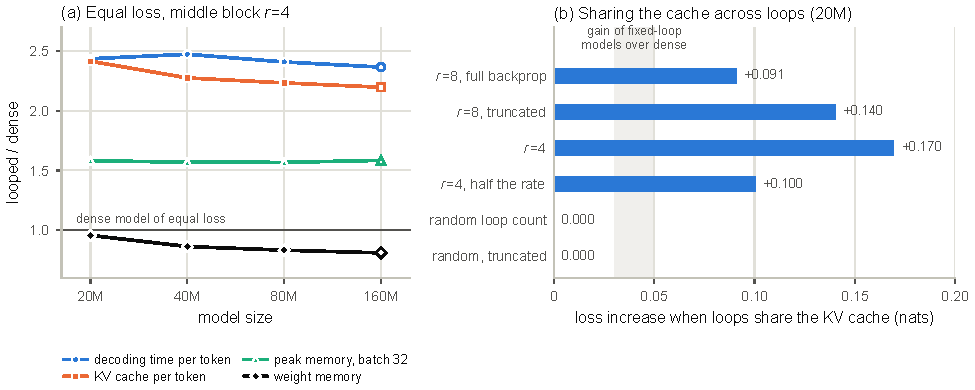
\includegraphics[width=\linewidth]{fig8_deployment}
  \caption{Deployment cost. \textbf{(a)}~A middle block looped 4 times against the dense model of equal loss at $40N$:
  ratios of decoding time per token (batch 1), KV cache per token, peak memory at batch 32 (1k context) and weight
  memory (open markers: 160M lies beyond the largest dense model). \textbf{(b)}~Sharing the KV cache across loops after
  training (20M, one cache slot per unique layer, written at a position's last loop): the loss increase on the main
  set; the shaded band is the fixed-loop models' gain over the dense model of the same size.}
  \label{fig:cost}
\end{figure}

At equal loss, the middle block looped 4 times needs 4\%, 14\%, 17\% and 19\% less weight memory than the dense model
from 20M to 160M (at 160M the dense model of equal loss is extrapolated beyond the largest one trained), but 2.20--2.41 times the KV cache per token and 2.37--2.47 times the decoding time, and its peak
memory at batch 32 is about 1.6 times that of the dense model. At batch 1 the larger KV cache cancels nearly all of the
saving in weights. In this range, loops save parameters, not latency or memory; the saving would grow where weights
dominate memory, for example one sequence with a short context in a much larger model, which we did not test.

Sharing the KV cache across loops would remove most of this cost. We applied terminal sharing, one cache slot per
unique layer written at a position's last loop and read by every later loop, to trained 20M models of one seed
(supplementary experiment S6, \lbl{pre-specified}; Figure~\ref{fig:cost}b). Every model that gains from its loops at this size loses two to four
times that gain: 0.09--0.17 nats against gains of 0.03--0.05 over the dense model, so with a shared cache it would fall
below the dense model of the same size. Truncated backpropagation does not make the cache shareable here, unlike in
\citet{huang2026towards}. The only models that share for free are those trained with a random loop count, whose block
contracts to a fixed point (Section~\ref{sec:mechanism}) and which gain nothing over the dense model. Among the fixed-loop
models, a lower learning rate loses less (0.100 against 0.170 with 4 loops). The likely ways to get sharing are
training towards convergence, or training with the shared cache, which \citet{monea2026shared} find costs no quality;
we tested neither.

\section{Discussion: when is recurrent depth test-time compute?}
\label{sec:discussion}

The same architecture behaves as a parameter-efficient model on text and as an extendable serial computer on the
chain task. We offer a reading of the difference. It is an interpretation of two settings, not
a tested law: in this reading, recurrent depth works as test-time compute when three conditions hold.

\paragraph{Headroom.} The model's errors must come from too few serial steps rather than from missing knowledge. On
the chain task the dense models know every table and fail only on depth; one more loop is one more step. On web text at
these sizes we found no sign of such errors: the per-token gain is a diffuse shift rather than a concentrated one, and
extra loops at inference never helped, at any learning rate (Sections~\ref{sec:where} and~\ref{sec:mechanism}). This is
the hardest of the three conditions to measure independently, since here it is inferred from where extra loops do and
do not help. The larger gains on math and code text hint at more headroom there, but at this size those sets are
dominated by which documents a run happened to see.

\paragraph{Extendable iteration.} The loop must be able to run longer without destroying its state. Which kind of
iteration a loop learns is decided by its training more than by the architecture. On text the same block becomes a
fixed-length program, a periodic cycle or a fixed point, depending on the loop schedule (Section~\ref{sec:mechanism}).
On the chain task the loop schedule decides whether the learned algorithm survives extra loops: models trained with as
many loops as steps lose their values when run longer, and a few random extra loops in training fix that; the learning
rate decides whether the task is learned at all (Sections~\ref{sec:probes}--\ref{sec:stopping}). A fixed point is
extendable but, on text, computes nothing more; a fixed-length program computes but cannot be extended.

\paragraph{A stopping signal.} Extra loops are only useful if the model can tell how many to run. On the chain task the
model's own confidence is such a signal for most regimes, and training a few loops past the last step makes the
regime that extends furthest stoppable as well (Section~\ref{sec:stopping}). We did not test stopping rules on text,
where extra loops did not help.

The chain task meets all three conditions once the model is trained for them; web text at these sizes showed no sign
of headroom, and its one extendable regime, the fixed point, gained nothing from running longer. Two follow-ups we did
not run would test this reading: a serial task whose input length does not grow with the number of steps, which would
also decide whether a written chain of thought extends when the prompt does not get longer; and training on text that
needs more serial steps, such as mathematics and code, compared at equal compute.

\paragraph{The value of a loop is not a constant of the architecture.} Even where the loop does not iterate, it buys
something on text, and what it buys depends on size and data: at 10--20M with up to 20 tokens per parameter a loop is
worth at most about its parameters, at 40M--160M with 20--40 tokens per parameter about 1.3--1.5 times them.
Effective-parameter laws whose loop gain depends on the loop count but not on model size or training tokens describe
the second regime well and the first not at all, and the single pre-registered $\varphi$ averaged over both. Studies at one scale will undersell or oversell the loop
depending on where they sit.

\paragraph{Practical guidance.} Within the range we measured:
\begin{itemize}
  \item Loop when parameters or data are the constraint, not compute or latency. The advantage at equal parameters
  grows with model size and tokens per parameter; at equal training compute a dense model was better in every
  measured comparison but one, a tie at the smallest size and the most data with the looped model's own learning rate; at deployment the loop pays its executed layers in decoding time and KV cache.
  \item Loop a middle block with full backpropagation, start with four loops on text, and judge at the target scale:
  at 40M--80M eight loops did about as well as four at about 1.75 times the training compute, and small-scale ablations undersell
  the loop.
  \item Tune the looped model's learning rate separately, especially at small scale and on tasks that need serial
  steps: at a learning rate that suits the dense model, most looped runs did not learn the chain task in the given
  steps.
  \item Do not expect test-time scaling on text from standard training. To see whether a model can use more loops,
  sweep the loop count at inference; to see whether it computes step by step even when it cannot, probe it.
  \item If a model must decide by itself how long to run, its confidence is a good stopping signal, and training a few
  loops past the last step makes the stop reliable. On our task, a written chain of thought was the cheaper choice
  within the training range and failed beyond it; that failure came from longer prompts, so it says little about tasks
  whose input length is fixed.
\end{itemize}

\section{Limitations}
\label{sec:limitations}

\begin{itemize}
  \item \textbf{Scale and evaluation.} Models of 10M--160M parameters with a 16k vocabulary, far below the sizes at which
  looped language models are deployed, evaluated by validation loss only, without downstream benchmarks. The trends
  with size may bend; there are five sizes, one seed at 80M and one looped cell at 160M.
  \item \textbf{Data.} One source, FineWeb-Edu, and one epoch. Data-limited or repeated-data regimes, where loops may
  matter more \citep{chen2026growth,gulbahar2026squeezing}, are not covered. Seeds change only the initialisation,
  except in the data-order experiment.
  \item \textbf{Equal compute.} 62 of the 320 equal-compute comparisons rest on an extrapolated dense loss, bracketed by
  two methods (Section~\ref{sec:equalcompute}), and the measured comparisons are not independent of each other.
  \item \textbf{Learning rates.} The dense rates come from a sweep at one budget; looped rates were re-tuned for one
  cell at 10M--40M with one seed (two at 20M), and the other cells and 80M--160M use the dense rates, which understated
  the looped model by up to 0.024 nats at 10M. On the synthetic task, several conditions tied at the top of the
  learning-rate criterion and the lowest rate was taken, while extrapolation is sensitive to the rate.
  \item \textbf{Single seeds} at 80M, for the random-loop language models, and for the KV-sharing test.
  \item \textbf{One synthetic task family.} The serial-task evidence comes from chains of table lookups and 6.6M-parameter
  looped models; extrapolation length varies widely across seeds. A pointer-chasing control was not learned and was
  dropped, and no dense control of equal executed depth was trained on text.
  \item \textbf{The comparison with a chain of thought} covers one task, models of 6.5M--29M parameters and one training
  recipe. Its prompt grows with the number of steps, so the chain of thought's failure beyond the training range is a
  failure to generalise to longer inputs, which the looped models handle on the same prompts; whether a written chain
  extends on a task whose input length does not grow was not tested. The chain-of-thought models got no help with length
  generalisation, and continuous thoughts \citep{hao2025training} were not tried.
  \item \textbf{Deployment} was measured on one GPU type, for models of at most 160M parameters, with one KV cache per
  executed layer; KV sharing was tested only as a change after training, at 20M.
  \item \textbf{Exploratory analyses.} The multiplier without a fitted law, the equal-compute bounds, the probes and the
  stopping comparison beyond the frozen rule were chosen after seeing data and are labelled as such; the pre-registered
  verdicts stand on their own.
\end{itemize}

\section{Pre-registration, deviations and reproducibility}
\label{sec:process}

The pre-registration, with the hypotheses, the grid, the fitting protocol and the decision rules, was frozen on
2026-09-23 before any training run, and its SHA-256 was committed to the repository the same day. The synthetic design
and its predictions were frozen on 2026-10-09, and the two supplementary plans on 2026-10-13 and 2026-10-15, each before
its runs. Every later change is dated in an append-only deviation log, together with its reason and its effect on the
conclusions; Appendix~\ref{app:deviations} summarises them. The most consequential were made before any comparison
between conditions: the synthetic task moved from modular arithmetic to lookup tables, and gained a curriculum, because
modular operations were not learnable at this size. Two reviews of the results (2026-10-14 and 2026-10-15) found five
errors and then about 35 errors and overstatements, among them a verdict judged with a quantity the frozen design did
not specify; all were corrected and logged before this paper was written. One evaluation that the
frozen design specified, the stopping rule of the loops = steps model, was computed but not reported until the second
review.

Code, configurations, the per-run results and training logs of all 232 language-model runs and 135 synthetic-task runs,
the fits, and the scripts that make every table and figure are available at \coderepo. Fits and figures run on a laptop
CPU; the model checkpoints (485 GB) are not included.

\paragraph{Use of AI assistance.}
The study was carried out with the help of an AI assistant (Claude, by Anthropic), which drafted code, analyses,
documents and this text under the direction of \theauthors. Every decision recorded in the pre-registration and the
deviation log, and responsibility for the content, lie with \theauthors. Every number in the paper is computed by
scripts in the repository.


\bibliography{references}
\bibliographystyle{tmlr}

\appendix
\section{The pre-registered hypotheses and decision rules}
\label{app:prereg}

The pre-registration (frozen 2026-09-23; an English translation of the binding original is in the repository with the
commands that verify its hash) fixed the grid of Section~\ref{sec:grid}, the fitting protocol of
Section~\ref{sec:measurement} and these decision rules. Before any data, three changes were made and dated in the
deviation log: the training data moved from sample-100BT to sample-10BT, which removed the $80N$ point of the 160M dense
model; the data point moved from the mean of a cooldown's last three evaluations to its final evaluation, the
three-point mean becoming a robustness variant (Table~\ref{tab:robust}); and a variant that counts $N$ without the output
head was added.

\begin{table}[h]
  \centering
  \caption{The four pre-registered hypotheses, their frozen decision rules and their verdicts.}
  \label{tab:verdicts}
  \footnotesize
  \begin{tabular}{p{0.19\linewidth}p{0.36\linewidth}p{0.36\linewidth}}
    \toprule
    Hypothesis & Decision rule for support & Verdict \\
    \midrule
    H1: truncated backpropagation lowers $\varphi$ & $\varphi_{\mathrm{trunc}} < \varphi_{\mathrm{full}}$ with
    non-overlapping 95\% bootstrap intervals, under both equal-token and equal-FLOP accounting; if only under equal
    tokens, the effect is attributed to the reallocation of FLOPs. & Not supported. Middle block 0.00 vs 0.13 (predicted
    direction, intervals overlap); whole stack 0.17 vs 0.00 (opposite direction). The equal-FLOP accounting agrees. \\
    H2: a looped middle block has a higher $\varphi$ than a looped whole stack & $\varphi_{\mathrm{mid}} >
    \varphi_{\mathrm{whole}}$ with non-overlapping intervals; raw-loss pairs of similar executed depth (middle block
    $r = 8$ vs whole stack $r = 4$; middle block $r = 4$ vs whole stack $r = 2$) are reported alongside, and a
    disagreement is reported as ``depends on the measure''. & Depends on the measure. $\varphi$ is mixed; raw losses at
    similar executed depth (36 against 32 and 20 against 16 layers) favour the middle block in 24 of 24 comparisons, by
    0.03--0.19 nats, less at larger sizes. \\
    H3: $\varphi$ saturates in $r$ & The geometric form has the lower extrapolation error in both directions (10M--40M
    predicting 80M; 20M--80M predicting 10M) and an information-criterion difference above 10. & Not supported. The
    geometric form predicts 80M from 10M--40M better (0.0085 vs 0.0096 rmse) and 10M from 20M--80M slightly worse
    (0.0203 vs 0.0200); the data do not separate the two forms. \\
    H4: the compute-optimal $r$ & Under matched training FLOPs the optimal $r \leq 2$, under matched deployment FLOPs
    larger; computed from the fitted law, without a test. & First half holds trivially (the dense model, $r = 1$, is
    optimal under training compute); second half not supported (it is optimal under deployment compute too). \\
    \bottomrule
  \end{tabular}
\end{table}

A factor effect counts only if it exceeds both the bootstrap half-width and the spread of $\varphi$ fitted separately
to the three seeds at 20M and 40M. The information criterion of H3 turned out to be computable only as a proxy from the
Huber loss, which is not a likelihood; it is not used as evidence (Appendix~\ref{app:deviations}). Two rules were added
during the grid, after the first spikes (2026-09-26) and after the collapse (2026-09-30), each before the results it
governs existed, and are dated in the deviation log: spikes are reported per run with a robustness fit without the runs that have them, and a cooldown result enters no fit
if its branch starts after a collapse or ends more than 1.0 nats above the lowest trunk loss before it (four results of
two runs: three of a 40M whole stack looped 8 times with truncation, seed 43, which collapsed, and the $10N$ result of a
40M whole stack looped 8 times with full backpropagation, seed 44, after a severe spike).

\section{Training details}
\label{app:training}

Table~\ref{tab:sizes} lists the sizes and Table~\ref{tab:supp} the supplementary experiments.

\begin{table}[h]
  \centering
  \caption{Model sizes and training settings on text. Size names give the approximate non-embedding parameters; $N$
  also counts the output head \citep{porian2024resolving}, which is large at small widths with a 16k vocabulary. The
  looped models of a size have the same unique layers plus a $2w^2$ injection map (under 2\% of $N$). The learning rate is that of the embedding and output layers, frozen after a
  33-run sweep; the hidden layers use $1.22$ times it. Warm-up is $2N$ tokens.}
  \label{tab:sizes}
  \small
  \begin{tabular}{lrrrrrl}
    \toprule
    Size & Width $w$ & Heads & $N$ & Tokens per step & Learning rate & Seeds (dense / looped) \\
    \midrule
    10M  & 320  & 5  & 15.4M  & 81,920  & $2.19\times10^{-3}$ & 3 / 3 \\
    20M  & 448  & 7  & 26.8M  & 131,072 & $1.53\times10^{-3}$ & 3 / 3 \\
    40M  & 640  & 10 & 50.1M  & 204,800 & $1.83\times10^{-3}$ & 3 / 3 \\
    80M  & 896  & 14 & 92.7M  & 327,680 & $2.03\times10^{-3}$ & 1 / 1 \\
    160M & 1280 & 20 & 179.6M & 524,288 & $1.56\times10^{-3}$ & 2 / 2 (middle block, $r=4$) \\
    \bottomrule
  \end{tabular}
\end{table}

\begin{table}[h]
  \centering
  \caption{The ten supplementary experiments, each run under a plan frozen before its runs (the S8 plan was written after
  the frozen stopping rule's results on the same checkpoints were known).}
  \label{tab:supp}
  \footnotesize
  \begin{tabular}{llll}
    \toprule
    & Plan frozen & What it adds & Where \\
    \midrule
    S1  & 2026-10-13 & Learning rates re-tuned for the dense model and a middle block looped 4 times & \S\ref{sec:multiplier}, App.~\ref{app:lr} \\
    S2  & 2026-10-13 & Learning rate and learning of the chain task, three seeds & \S\ref{sec:lrsynthetic} \\
    S3  & 2026-10-13 & Inference cost & \S\ref{sec:cost}, App.~\ref{app:cost} \\
    S4  & 2026-10-15 & Dense models continued to $640N$ (10M) and $320N$ (20M) & \S\ref{sec:equalcompute}, App.~\ref{app:lr} \\
    S5  & 2026-10-15 & Chain of thought and pause tokens on the chain task & \S\ref{sec:inrange}, \S\ref{sec:extension} \\
    S6  & 2026-10-15 & KV cache shared across loops after training & \S\ref{sec:cost}, App.~\ref{app:cost} \\
    S7  & 2026-10-15 & Data order & \S\ref{sec:mechanism}, App.~\ref{app:fits} \\
    S8  & 2026-10-15 & Answer-free stopping rules & \S\ref{sec:stopping}, App.~\ref{app:synthetic} \\
    S9  & 2026-10-15 & Loops = steps with 0--4 random extra loops & \S\ref{sec:stopping} \\
    S10 & 2026-10-27 & Dense models with 18 layers and the looped model's parameters & \S\ref{sec:depth}, App.~\ref{app:s10} \\
    \bottomrule
  \end{tabular}
\end{table}

\paragraph{Data.} The three further validation sets of 20M tokens each come from a 6B-token sample of SlimPajama, from
FineMath (finemath-4plus) and from GitHub code (github-code-clean,
\url{https://huggingface.co/datasets/codeparrot/github-code-clean}).

\paragraph{Extensions.} The extensions continue the 10M middle blocks looped 4 and 8 times (two seeds) to $80N$ and
$160N$, a 10M whole stack looped 4 times and a truncated one looped 8 times (one seed) to the same budgets, the 10M dense
model to $160N$ and the 20M middle blocks looped 4 and 8 times (two seeds) to $80N$.

\paragraph{Learning rates.} A sweep of 33 runs at $10N$ (30 dense runs at five rates per width, a $\beta_2 = 0.99$ group
at 20M, and three looped runs at 80M) fixed the rate per width (Table~\ref{tab:sizes}); the minima of all five widths
lie inside the swept range, and $\beta_2 = 0.95$ beat 0.99 by 0.008 nats. The hidden layers use
$\eta_0 (8/12)^{-1/2} \approx 1.22\,\eta_0$. A check for looped cells, whose decision rule was written before its runs on 2026-09-25, two days after the
pre-registration (20M, ten cells at 0.5, 0.71 and 1
times the dense rate, $10N$) found no better rate by the rule fixed in advance (pooled best multiple 0.97, threshold
0.84), so all looped language models use the dense rates. Nine of the ten cells were best at 1$\times$, the top
of that range, so higher rates were not excluded. The residual scaling of Section~\ref{sec:models} is meant to keep the
best rate independent of $r$: we found no downward shift of the best rate in this check, but at 10M with longer training
the looped model preferred lower rates (Section~\ref{sec:multiplier}).

\paragraph{FLOP accounting.} Training FLOPs count two FLOPs per multiply-add over every executed layer, the attention
terms and the output head, plus a backward pass of twice the forward cost for every layer that receives gradients; with
truncated backpropagation the backward pass covers the prelude, the coda, the output head and the last $r/2$ loops.

\paragraph{The grid at equal parameters.} Table~\ref{tab:gaps} gives the looped minus dense loss per cell and size,
averaged over the three budgets.

\begin{table}[h]
  \centering
  \caption{Looped minus dense loss at equal parameters and tokens, mean over the budgets $10N$, $20N$ and $40N$ and over
  seeds (negative: looped better). $^{*}$Includes a seed with a severe loss spike; without it, $-0.029$.}
  \label{tab:gaps}
  \small
  \begin{tabular}{lcccc}
    \toprule
    Cell & 10M & 20M & 40M & 80M \\
    \midrule
    Middle block, $r=2$ & $+0.068$ & $+0.025$ & $-0.010$ & $-0.015$ \\
    Middle block, $r=4$ & $+0.055$ & $+0.002$ & $-0.030$ & $-0.039$ \\
    Middle block, $r=4$, truncated & $+0.079$ & $+0.031$ & $+0.006$ & $+0.009$ \\
    Middle block, $r=8$ & $+0.031$ & $-0.003$ & $-0.033$ & $-0.033$ \\
    Middle block, $r=8$, truncated & $+0.039$ & $+0.001$ & $-0.022$ & $-0.018$ \\
    Whole stack, $r=2$ & $+0.172$ & $+0.079$ & $+0.021$ & $+0.003$ \\
    Whole stack, $r=4$ & $+0.150$ & $+0.085$ & $+0.047$ & $+0.025$ \\
    Whole stack, $r=4$, truncated & $+0.044$ & $+0.003$ & $-0.014$ & $+0.017$ \\
    Whole stack, $r=8$ & $-0.074$ & $-0.055$ & $+0.213^{*}$ & $-0.003$ \\
    Whole stack, $r=8$, truncated & $-0.053$ & $-0.041$ & $-0.042$ & $-0.020$ \\
    \bottomrule
  \end{tabular}
\end{table}

\paragraph{Two observations from the grid.} Truncated backpropagation, predicted to hurt, helped whole-stack loops with
four loops at every size (Table~\ref{tab:gaps}): at 20M a whole stack looped 4 times reached 3.646 with truncation and
3.783 with full backpropagation at $10N$ (three-seed means); with eight loops it was slightly worse at 10M--20M. At 10M
the only looped cells better than the dense model on average over the three budgets were whole-stack loops with
$r = 8$. Truncation and whole-stack loops also brought instability: 30 of the 111 runs had at least one loss spike, 25
with truncated backpropagation (16 of these whole-stack loops) and five whole-stack loops with $r = 8$ and full
backpropagation; one run collapsed. In an exploratory follow-up, a 10M whole stack looped 4 times with truncation,
trained at half the learning rate in three seeds, had no spike at all (4, 1 and 10 at the original rate); it was worse
by 0.044 nats at $10N$ and better by 0.064 at $40N$, which cannot be credited to the missing spikes alone, since longer
budgets also favour a lower constant rate.

\section{Fits and robustness}
\label{app:fits}

The fits use a Huber loss in log space ($\delta = 10^{-3}$), 500 random starts and 1000 block-bootstrap resamples. The
primary ruler, fitted to 54 dense results, is $E = 0.050$ (at the lower bound of the fit), $A = 6.98$,
$\alpha = 0.054$, $B = 1065$, $\beta = 0.370$; the joint fit over all 352 results gives $E = 1.94$, $A = 61.7$,
$\alpha = 0.267$, $B = 197$, $\beta = 0.266$. Under the constant-$\varphi$ model, setting every $\varphi$ to 0 raises the
Huber loss only from 0.00352 to 0.00379, and setting it to 1 raises it to 0.0142. Table~\ref{tab:robust} gives the
primary $\varphi$ under the robustness variants of the pre-registration and of the deviation log, each fixed before the
results it governs. Fitted separately to each seed, $\varphi$ varies by
0.10--0.21 per cell at 20M and 0.00--0.11 at 40M; the factor effects of Table~\ref{tab:prereg} (0.13--0.17) do not exceed
the 20M spread.

\begin{table}[h]
  \centering
  \caption{$\varphi$ (primary fit) under robustness variants, in the order middle block full / middle block truncated /
  whole stack full / whole stack truncated.}
  \label{tab:robust}
  \small
  \begin{tabular}{ll}
    \toprule
    Variant & $\varphi$ \\
    \midrule
    Primary analysis & 0.13 / 0.00 / 0.00 / 0.17 \\
    Without the 30 runs with loss spikes & 0.13 / 0.11 / 0.00 / 0.22 \\
    Mean of the last three evaluations (the pre-registered data point) & 0.14 / 0.00 / 0.00 / 0.17 \\
    Second validation set (SlimPajama) & 0.31 / 0.18 / 0.02 / 0.30 \\
    Without $r = 8$ & 0.07 / 0.00 / 0.00 / 0.07 \\
    Half the budget & 0.08 / 0.00 / 0.00 / 0.15 \\
    $N$ without the output head & 0.07 / 0.00 / 0.00 / 0.14 \\
    Equal-FLOP accounting & 0.13 / 0.08 / 0.00 / 0.16 \\
    \bottomrule
  \end{tabular}
\end{table}

For H3, the pre-registered extrapolation (10M--40M to 80M and 20M--80M to 10M, with the dense-only 160M size in neither
training set) gives a root-mean-square error of 0.0096 and 0.0200 for $r^{\varphi}$ and 0.0085 and 0.0203 for the
geometric form. Five of the seven robustness variants show the same split; without $r = 8$ the split is reversed, and
on the second validation set $r^{\varphi}$ is better in both directions. For H4, the fitted law makes the dense model
optimal at every training budget from $10^{17}$ to $10^{20}$ FLOPs, with the smallest available $r$ the best looped
choice, 0.00--0.17 nats behind; under deployment compute the dense model is optimal as well, with either set of ruler
parameters.

\paragraph{Loop-by-loop probes of the language models.} The state after each loop $k$ is read in three ways: with the
model's own output layers (the logit lens of \citealp{nostalgebraist2020logit}, which here is the same as running the
model with $k$ loops), with a learned linear $w\times w$ map in front of the output layers (in the spirit of the tuned
lens of \citealp{belrose2023tuned}, but trained on the next token rather than distilled from the model's own output),
and with a learned linear head; the maps are trained on 10M unseen training tokens and evaluated on 2M tokens of the
main validation set.

\paragraph{The multiplier plane.} A least-squares plane in $\log_2 M$ over the middle block looped 4 times gives a
factor of 1.21 per doubling of model size and 1.14 per doubling of tokens per parameter (1.16 with 8 loops), with
classical 95\% intervals, which include the plane's misfit, of 1.13--1.30 and 1.05--1.24; by these intervals the product
term is indistinguishable from zero. On the plane the loop breaks even ($M = 1$) at about $N = 35$M with 20 tokens per
parameter and at about $N = 12$M, below the smallest model, with 80; the measured points agree at 80 (1.04 for the 10M
model, 1.05 on the plane) but reach $M = 1$ earlier at 20 (the 20M model is at 0.99, the plane at 0.93). At 10M with 10
tokens per parameter the two dense models measured at that number of tokens are out of order (the 20M one, at 5.7
tokens per parameter, is worse than the 10M one), so $\Nstar$ cannot be extrapolated either.

\paragraph{Published multipliers.}\label{app:published} Published equal-parameter results mostly restate to a similar range in comparable settings, and to higher values at
larger sizes or with far more tokens per parameter. Where a paper reports a non-looped ladder, we interpolate it in the
same way. Parcae's models, trained with a loop count sampled around a mean of 8 and backpropagated through 4 of them,
and run with 8, are worth 1.31--1.46 dense parameters per parameter at 140M--770M \citep{prairie2026parcae}, against a
ladder trained on the same tokens per parameter, which understates the value. Ouro's models looped 4 times are worth
1.23 and 1.36 at 134M and 374M (about 150 and 50 tokens per parameter) and more than 1.75 at 778M, beyond its largest
non-looped model, but less than their parameters at 53M despite about 380 tokens per parameter, measured by mean
benchmark accuracy read off a plot (\citealp[App.~D.1]{zhu2025scaling}). The two 12-layer looped models of \citet{saunshi2025reasoning}, about 0.5B
parameters looped 2 and 4 times, are worth 1.26 and 1.36, and their shallower blocks looped 3, 4 and 6 times
1.47--1.95, at about 750--1500 tokens per parameter. The law of \citet{schwethelm2026how} ($\varphi = 0.46$, 95\% interval 0.41--0.53) implies 1.25, 1.45 and 1.56
for 2, 4 and 8 loops in their iso-depth layouts. These studies differ from ours in size, data and recipe, so the
agreement is a consistency check, not a pooled estimate. They barely sample models below 40M trained on 20 or fewer
tokens per parameter, where we find a model with a looped middle block worth at most about as many dense
parameters as it has. That the value rises with tokens per
parameter at equal parameters is a dependence that effective-parameter laws whose loop gain depends on the loop
count (and, for mixtures of experts, on the sparsity) but not on the training tokens
\citep{schwethelm2026how,chen2026moe} do not capture; it agrees with the recommendation of \citet{prairie2026parcae} to
increase looping and data in tandem, and with the finding of \citet{chen2026growth} that with repeated data the best
loop count grows with compute.

\paragraph{Where the gain lands, and what the seeds measure.} Per token, the gain on web text is a small, broad shift:
about half of the tokens improve, and the gain is not concentrated on hard tokens beyond what two dense seeds differ by
\lbl{(exploratory)}. On math and code text the gain is larger, on average about 3 and 7 times the gain on the main set,
but the seed-to-seed spread on those sets is 10--100 times larger as well. Supplementary experiment S7
\lbl{(pre-specified)} showed that the code set is even more sensitive to the data order, which our seeds share, than to
the initialisation (the math set is not): at 20M, training the same initialisation on three disjoint parts of the data
stream moves the main-set loss by only 0.003--0.011 nats, 0.1--0.5 times the spread between initialisation seeds (the plan
had predicted one to three times), but moves the code-set loss by 0.21--0.69 nats, up to 7 times that spread, and changes
the sign of the looped-minus-dense gap there. Of the plan's four predictions only this one, a code-set spread above 0.1,
held: on the main set the data-order spread was smaller than predicted relative to the initialisation spread (and, for
the dense model, below the predicted 0.005--0.02 nats), and the looped-minus-dense gap did not vary less than the losses. Both the initialisation and the documents a run happens to see move its out-of-distribution loss strongly at this
size, so we draw no conclusions from differences on those sets.

\section{Learning rates (S1) and equal compute at the largest budgets (S4)}
\label{app:lr}

S1 re-tuned the dense model and the middle block looped 4 times at 10M, 20M and 40M: 0.5 to 1.41 times the dense rate,
plus 0.35 times where the best rate lay at the lowest one tried, at $10N$--$40N$ (at 10M also $80N$ and $160N$), with one
seed (two at 20M). Table~\ref{tab:s1} gives the gap between the middle block looped 4 times and the dense model at the
shared rate
($\Delta_1$) and with each model at its best rate ($\Delta^{\star}$), and $h = \Delta_1 - \Delta^{\star}$, the bias of
the shared rate against the looped model. The pre-specified readings: the trend with size holds (at $40N$ the
improvement from 10M to 40M is 0.050 against 0.065 at the shared rate, above the threshold of half of it), the trend
with data holds and grows (10M from $10N$ to $160N$: 0.141 against 0.119), the equal-compute verdict was unchanged
at the time (its 10M comparison at $160N$, extrapolated then, was later measured in S4: $-0.011$, a looped advantage, and
$+0.005$ with a second seed; Section~\ref{sec:equalcompute}), and
the bias exceeds the 0.01 tolerance at 10M only.

\begin{table}[h]
  \centering
  \caption{S1: looped (middle block, $r = 4$) minus dense loss at the shared rate and at each model's best rate (seed 42;
  20M: mean of seeds 42 and 43). $^{\dagger}$The lowest rate tested.}
  \label{tab:s1}
  \small
  \begin{tabular}{lcccc}
    \toprule
    Size, budget & $\Delta_1$, shared rate & $\Delta^{\star}$, best rates & $h$ & Best rate, dense / looped \\
    \midrule
    10M, $10N$  & $+0.082$ & $+0.082$ & $+0.000$ & 1 / 0.71 \\
    10M, $20N$  & $+0.044$ & $+0.026$ & $+0.018$ & 1 / 0.5 \\
    10M, $40N$  & $+0.015$ & $-0.005$ & $+0.020$ & 1 / 0.5 \\
    10M, $80N$  & $-0.010$ & $-0.035$ & $+0.024$ & 1 / 0.35$^{\dagger}$ \\
    10M, $160N$ & $-0.037$ & $-0.059$ & $+0.022$ & 1 / 0.35$^{\dagger}$ \\
    20M, $10N$  & $+0.028$ & $+0.028$ & $0.000$ & 1 / 1 \\
    20M, $20N$  & $-0.005$ & $-0.005$ & $0.000$ & 1 / 1 \\
    20M, $40N$  & $-0.031$ & $-0.031$ & $0.000$ & 1 / 1 \\
    40M, $10N$  & $-0.008$ & $-0.008$ & $0.000$ & 1 / 1 \\
    40M, $20N$  & $-0.032$ & $-0.036$ & $+0.004$ & 1 / 0.71 \\
    40M, $40N$  & $-0.050$ & $-0.055$ & $+0.005$ & 0.71 / 0.71 \\
    \bottomrule
  \end{tabular}
\end{table}

On the trunk checkpoints at $32N$, the range of the main-set loss over 4--16 inference loops is 0.30, 0.36, 1.02, 3.39
and 4.10 nats at 0.35, 0.5, 0.71, 1 and 1.41 times the dense rate at 10M, 0.53--3.42 at 20M and 0.77--4.81 at 40M
(0.5 to 1.41 times): lower rates make the iteration closer to convergent, but at every rate the better of 8 and 16 loops
is worse than the 4 loops of training, by 0.07--3.0 nats.

\paragraph{Extrapolated equal-compute comparisons.} Two extrapolations bracket a dense loss beyond the measured curve:
in a backtest that drops the last budgets of every measured dense curve, extending the last segment predicts a dense
loss 0.023--0.036 nats too low one doubling out (it flatters the dense model), and a power law fitted to the whole curve
one 0.006--0.027 too high (it flatters looping). After S4, 62 equal-compute comparisons still need an extrapolated dense
loss: 43 at 40M--160M, and 19 at 10M--20M, almost all for the third seed, whose dense curve ends at $80N$. At 160M and
$40N$ the bracket reaches from $+0.004$ to $+0.043$.

\paragraph{Equal compute at the largest budgets (S4).} Table~\ref{tab:equalcompute} gives the equal-compute comparisons at the
largest looped budgets. The S4 plan had predicted gaps between $-0.01$ and $+0.04$, the dense model ahead in most and none
below $-0.02$; the last two held, but four of the nine measured top-budget gaps exceeded $+0.04$ (up to $+0.054$).

\begin{table}[h]
  \centering
  \caption{The equal-compute comparisons at the largest looped budgets (S4; looped minus dense loss on the main
  validation set, means over two seeds; negative: looped better). At equal compute the dense model is trained on 2.2--3.8
  times the tokens.}
  \label{tab:equalcompute}
  \footnotesize
  \begin{tabular}{lccc}
    \toprule
    & Training FLOPs & \multicolumn{2}{c}{Looped $-$ dense loss} \\
    \cmidrule(lr){3-4}
    Looped cell (size, tokens per parameter) & vs dense & equal parameters and tokens & equal compute \\
    \midrule
    Middle block, $r=4$ (10M, $160N$) & 2.2$\times$ & $-0.033$ & $+0.016$ \\
    Middle block, $r=8$ (10M, $160N$) & 3.7$\times$ & $-0.051$ & $+0.034$ \\
    Middle block, $r=4$ (20M, $80N$)  & 2.2$\times$ & $-0.051$ & $+0.022$ \\
    Middle block, $r=8$ (20M, $80N$)  & 3.8$\times$ & $-0.064$ & $+0.052$ \\
    \midrule
    Middle block, $r=4$, 0.35$\times$ rate (10M, $160N$) & 2.2$\times$ & --- & $-0.011$, $+0.005$ (seeds) \\
    \bottomrule
  \end{tabular}
\end{table}

\section{Depth or sharing (S10)}
\label{app:s10}

The plan was frozen on 2026-10-27, before any of its runs. Dense models with 18 layers and the looped model's number of
parameters (Table~\ref{tab:s10}) were trained with the recipe of the grid's runs of the same size: the same data in the
same order, batch, warm-up and optimiser settings, one constant-rate trunk with cooldown branches ending at $10N$, $20N$
and $40N$ of that size (in tokens identical to the looped runs), the same evaluation sets, and seeds 42, 43 and 44. The
embedding and output layers use the frozen rate of their width ($2.19\times10^{-3}$ at width 320, $1.53\times10^{-3}$ at
448) and the hidden layers $(18/12)^{-1/2}$ times it, as the code does for any depth; seed 42 was also trained at 0.71
and 1.41 times that rate. Training FLOPs per token are 205M (dense, 8 layers), 456M (looped) and 239M (dense, 18 layers)
at 20M, and 364M, 835M and 406M at 40M. None of the ten runs had a loss spike.

\begin{table}[h]
  \centering
  \caption{S10: dense models with 18 layers ($18 \times 320$, $N = 28.1$M; $18 \times 448$, $N = 51.2$M) against the
  middle block looped 4 times (8 unique layers, 20 executed; $N = 27.2$M and 51.0M), at the rule's learning rate. Losses
  and gaps are means over three seeds (the gap per seed in parentheses; positive: looped better); $M$ is read off the
  8-layer dense ruler; 95\% intervals from resampling seeds. At 20M the plan reports the results descriptively:
  $M_{\mathrm{loop}}$ is near 1 at $10N$ and $20N$, and $R$ is unstable (0.58, 10.1 and $-0.40$).}
  \label{tab:s10}
  \footnotesize
  \setlength{\tabcolsep}{2.6pt}
  \begin{tabular}{lcccccc}
    \toprule
    Size, budget & Dense, 18 layers & Looped & Gap (seeds) & $M_{\mathrm{deep}}$ & $M_{\mathrm{loop}}$ & $R$ \\
    \midrule
    20M, $10N$ & 3.654 & 3.671 & $-0.017$ ($-0.010$, $-0.016$, $-0.026$) & 0.84 [0.76, 0.98] & 0.74 [0.67, 0.83] & --- \\
    20M, $20N$ & 3.465 & 3.456 & $+0.008$ ($+0.017$, $+0.013$, $-0.005$) & 0.92 [0.85, 1.01] & 0.99 [0.92, 1.11] & --- \\
    20M, $40N$ & 3.335 & 3.307 & $+0.028$ ($+0.037$, $+0.033$, $+0.015$) & 0.94 [0.89, 1.00] & 1.16 [1.09, 1.25] & --- \\
    40M, $10N$ & 3.397 & 3.394 & $+0.003$ ($+0.004$, $+0.004$, $-0.001$) & 1.10 [1.04, 1.14] & 1.15 [1.08, 1.20] & 0.67 [0.43, 1.03] \\
    40M, $20N$ & 3.232 & 3.217 & $+0.015$ ($+0.017$, $+0.018$, $+0.010$) & 1.11 [1.09, 1.13] & 1.26 [1.21, 1.29] & 0.46 [0.38, 0.55] \\
    40M, $40N$ & 3.119 & 3.090 & $+0.029$ ($+0.030$, $+0.032$, $+0.026$) & 1.11 [1.10, 1.12] & 1.34 [1.31, 1.36] & 0.36 [0.32, 0.41] \\
    \bottomrule
  \end{tabular}
\end{table}

\paragraph{Readings fixed in advance.} The primary reading is $R$ at 40M averaged over the three budgets: at least 0.75
reads as ``most of the advantage is a depth effect'', 0.25--0.75 as ``partly depth, partly sharing'' and below 0.25 as
``looping buys more than depth''. It is 0.50 (95\% interval 0.41--0.62). The plan would also have reported the two
models as on par at 40M had the gap been within 0.01 nats at all three budgets; it is not ($+0.015$ and $+0.029$ at $20N$
and $40N$).

\paragraph{Learning rate.} Seed 42 at 0.71, 1 and 1.41 times the rule's rate: at 40M 3.421, 3.396 and 3.382 at $10N$,
3.246, 3.231 and 3.225 at $20N$, and 3.126, 3.118 and 3.117 at $40N$; at 20M the rule's rate was the best at every
budget. Because 1.41 times the rate beat the rule's rate by more than 0.01 nats at 40M and $10N$ (by 0.014), the plan
asks for the readings also at the best rate tried, as in S1, the primary reading staying at the rule's rate. With each
model at its best tested rate (seed 42; the looped model's best rates, from S1, are 1, 0.71 and 0.71 times the dense
rate at $10N$, $20N$ and $40N$; both read off the 8-layer dense runs at their frozen rates, seed means, with
\texttt{fit/supp3\_best\_lr.py}), the gap is $-0.010$, $+0.015$ and $+0.036$, $M_{\mathrm{deep}}$ 1.37, 1.17 and 1.12,
$M_{\mathrm{loop}}$ 1.18, 1.33 and 1.41, and $R$ 1.91, 0.56 and 0.34 (mean 0.94; for seed 42 at the rule's rate 0.58,
0.45 and 0.37, mean 0.47). The mean at the best rates falls in the band the plan reads as ``most of the advantage is a depth effect''; it is
carried by $10N$, where $\log M_{\mathrm{loop}}$ is smallest, and the primary reading stays at the rule's rate.
The analysis script written before the results flagged this case but did not compute these readings; they come from a
script written afterwards that implements the rule of the plan.

\paragraph{Predictions.} The plan predicted $R$ at 40M between 0.25 and 0.75 (held: 0.50); the 18-layer dense model
better than the 8-layer one of the same size by 0.01--0.03 nats at 40M (0.007, 0.016 and 0.020 at $10N$, $20N$ and $40N$:
held at two of the three budgets; at 20M it is worse by 0.014, 0.008 and 0.003); and the rule's rate within 0.01 nats of
the best of the three (held at five of the six budgets).

\paragraph{Equal compute \lbl{(exploratory)}.} Read as in Section~\ref{sec:equalcompute}, without extrapolation: the
looped model is behind the 18-layer dense model of equal training compute by 0.166 nats at 40M and $10N$ (compute ratio
2.05) and by 0.193 and 0.112 at 20M and $10N$ and $20N$ (ratio 1.91).

\section{Deployment measurements}
\label{app:cost}

Inference was timed on one RTX 4090 (all other GPUs idle) in bf16, with the decoding step in a CUDA graph, one KV-cache
slot per executed layer, random weights, a 512-token prompt and 512 generated tokens, at batch 1 and 32. Table~\ref{tab:s3} gives the ratios at
equal loss for all middle-block and whole-stack cells, against the dense model that reaches the same loss at $40N$
(interpolated between dense sizes).

\begin{table}[h]
  \centering
  \caption{S3: looped over dense, at equal loss. $^{*}$160M lies beyond the largest dense model (extrapolated).}
  \label{tab:s3}
  \footnotesize
  \setlength{\tabcolsep}{4pt}
  \begin{tabular}{llccccc}
    \toprule
    & & Weight & KV cache & Decoding time & \multicolumn{2}{c}{Peak memory} \\
    \cmidrule(lr){6-7}
    Cell & Sizes & memory & per token & batch 1 & batch 1 & batch 32 \\
    \midrule
    Middle block, $r=2$ & 20M--80M  & 0.93--1.03 & 1.43--1.51 & 1.45--1.49 & 0.99--1.15 & 1.21--1.24 \\
    Middle block, $r=4$ & 20M--160M & 0.81$^{*}$--0.96 & 2.20--2.41 & 2.37--2.47 & 0.98$^{*}$--1.20 & 1.57--1.58 \\
    Middle block, $r=8$ & 20M--80M  & 0.83--0.92 & 4.01--4.23 & 4.27--4.56 & 1.08--1.34 & 2.29--2.40 \\
    Whole stack, $r=4$  & 20M--80M  & 1.03--1.11 & 4.02--4.27 & 4.00--4.11 & 1.18--1.84 & 2.32--2.41 \\
    Whole stack, $r=8$  & 20M--80M  & 0.81--0.85 & 6.96--7.23 & 7.57--7.91 & 1.27--1.50 & 3.38--3.91 \\
    \bottomrule
  \end{tabular}
\end{table}

For KV sharing (S6), the first 262{,}144 tokens of the main validation set were decoded token by token in 256 windows of
1024, with one cache slot per executed layer (whose loss equals that of the ordinary forward pass to four decimals) and
with one slot per unique layer, written at a position's last loop and read by every later loop. The models are the 20M
trunk checkpoints at $32N$ (seed 42); Figure~\ref{fig:cost}b gives the loss differences, and the random-loop model run
with 16 loops instead of 8 also shares at no cost.

At batch 1 the larger KV cache cancels the saving in weights: the looped model needs 1--2\% less peak memory at
80M--160M and more at 20M--40M (up to 1.2 times). In this range, loops save parameters, not latency or memory;
the saving would grow where weights dominate memory, for example one sequence with a short context in a much larger
model, which we did not test. Truncated backpropagation does not make the cache shareable here, unlike in \citet{huang2026towards}. Among the
fixed-loop models, a lower learning rate loses less (0.100 against 0.170 with 4 loops). The S6 plan had predicted
that the fixed 8-loop model would break (a loss increase above 0.3) and the truncated one would lose less than 0.1;
the increases were 0.09 and 0.14, while the random-loop models shared at no cost and the lower learning rate lost
less, as predicted (two of four).

\begin{figure}[h]
  \centering
  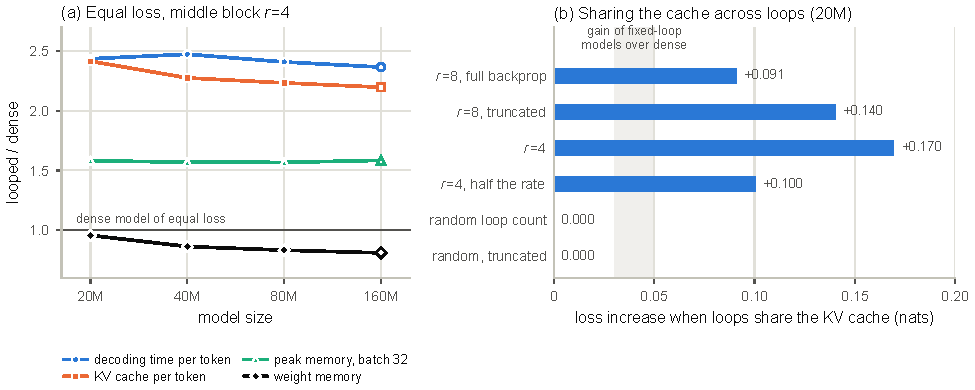
\includegraphics[width=\linewidth]{fig8_deployment}
  \caption{Deployment cost. \textbf{(a)}~A middle block looped 4 times against the dense model of equal loss at $40N$:
  ratios of decoding time per token (batch 1), KV cache per token, peak memory at batch 32 (1k context) and weight
  memory (open markers: 160M lies beyond the largest dense model). \textbf{(b)}~Sharing the KV cache across loops after
  training (20M, one cache slot per unique layer, written at a position's last loop): the loss increase on the main
  set; the shaded band is the fixed-loop models' gain over the dense model of the same size.}
  \label{fig:cost}
\end{figure}

\section{The synthetic task}
\label{app:synthetic}

\paragraph{Data and training.} Tokens are the values 0--96 and a few markers (start, separator, lookup, answer and
padding); a problem is a start value followed by $d$ steps of the form \texttt{LUT k ;}, with the table index $k$
written as one of the value tokens 0--31, and the answer marker. Problems are drawn online. During
the first half of training the largest step count grows linearly from 1 to 8; the second half draws uniformly from
1--8. Models have width 256 and attention heads of dimension 64, and the looped models use the input injection and
residual scaling of the language models. Training uses AdamW ($\beta = (0.9, 0.95)$, weight decay 0.1, gradient clipping
1.0), 400 warm-up steps and a cosine decay to a tenth of the peak rate, 512 problems per step, 32{,}000 steps. The two
deepest conditions of S5 and S9 accumulated gradients over two half-batches to fit in memory (the same loss and update).
Probes are linear maps from the state after each loop (or layer) to the 97 values, trained on 4000 problems with 8 steps
and tested on 1000, at the table-index, separator and next-operation positions of each step, keeping the best.

\paragraph{Learning rates.} The sweep (seed 1; $2.5\times10^{-4}$, $5\times10^{-4}$ and $10^{-3}$, extended at an
edge) chose by mean in-range accuracy at the condition's own loop count: dense 8 and 20 layers $10^{-3}$, dense 36 layers
$5\times10^{-4}$, looped $r = 2$ and $r = 8$ $2.5\times10^{-4}$, looped $r = 4$, random loop count, loops = steps, the S9
model and the chain-of-thought models $1.25\times10^{-4}$, the pause model $5\times10^{-4}$. These are the rates of the
embedding and output layers; the hidden layers use $(L/12)^{-1/2}$ times them, with $L$ the number of unique layers (1.22, 0.77 and 0.58 for 8, 20 and 36), so the hidden layers of the 36-layer
dense model train at about the rate of the 2- and 8-loop models. The criterion saturates at low rates (the loops = steps model scored 0.9999 at three rates and the chain-of-thought models
1.000 at all four), such ties went to the lowest rate by implementation, a rule the protocol had not specified, and the
4-loop, random-loop and S9 models were best at the lowest rate tried. Extrapolation is sensitive to this choice: in the
sweep, the accuracy of the loops = steps model on 9 to 14 steps fell from 1.00 to 0.91 at $2.5\times10^{-4}$ but to 0.05
at $1.25\times10^{-4}$.

\paragraph{Probes.} The \emph{frontier} is the first loop at which each value becomes decodable (probe accuracy
$\geq 0.5$), and \emph{persistence} is the lowest probe accuracy a value reaches in the loops after that, averaged
over the values (Figure~\ref{fig:probes}). In 5 of the 10 seeds of the 20- and 36-layer dense models no
intermediate value after the first appears at the step positions: four show only $x_1$ (probe accuracy 0.50--0.74)
and, at the last layer, the answer, and one shows nothing. Measured by the share of values that first become
decodable at their own loop, a reading of the design's diagonal share fixed after the results, the loops = steps and
8-loop models are diagonal (0.95 and 0.975) and the others are not (0.125); read as the share decoded most accurately
at their own loop, they are 0.625 and 0.425.


\paragraph{S2.} Its plan identified the conditions with 4 and 8 loops, the random loop count and loops = steps as
extrapolating and left out $r = 2$ on the strength of a number corrected later (Appendix~\ref{app:deviations}). Probes of
all sweep checkpoints \lbl{(exploratory)} show the step-by-step frontier at rates up to $5\times10^{-4}$ and not above, for 4 and 8 loops and the random loop
count alike. At $10^{-3}$ the runs that did not learn the training range reached 0.49--0.98 in range; at $5\times10^{-4}$
the runs that learned it extended about as far as the formal runs (8 loops: 2.7
steps beyond the range against 3.2; loops = steps: 4.0 against 4.8), except the random loop count (2 against 4.2).

\paragraph{Where the chain of thought breaks.} As soon as the prompt holds more than 8 tables, the first wrong token
of the 8-layer chain-of-thought model is one of the first three written ones in 97--98\% of the problems, and even
when the correct earlier tokens are given, the tokens after the first two are mostly wrong (accuracy 0.04--0.10)
\lbl{(exploratory)}.

\paragraph{Stopping rules.} Figure~\ref{fig:stopping} shows the confidence rule against the chain length. The plan's selection rule, the highest accuracy over 9--16 steps
on the selection set among rules that keep the in-range accuracy within 0.01 of the training loop count's, also
admitted votes over loop counts and picked a vote for three of the five conditions; without votes it picks the 0.5\%
state rule for $r = 4$, the confidence rule at 0.99 for $r = 8$ and the random loop count, and at 0.9 for $r = 2$; for S9
it picks the 0.5\% state rule with or without votes. Where it picked a vote, the vote runs all 32 loops and comes within
0.013 of the best fixed count without beating it.

\begin{figure}[h]
  \centering
  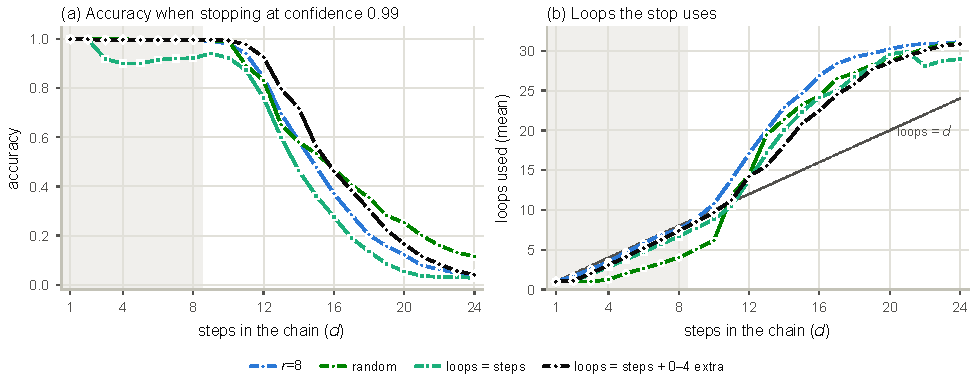
\includegraphics[width=\linewidth]{fig7_stopping}
  \caption{Stopping when the model's top probability reaches 0.99 (reporting set, mean over five seeds).
  \textbf{(a)}~Accuracy. \textbf{(b)}~Loops used: the stop runs few loops on short chains and many on long ones. The
  model trained with loops = steps loses part of the training range; trained with a few random extra loops, it keeps the
  training range and stops best of the four beyond it, up to 15 steps.}
  \label{fig:stopping}
\end{figure}

\paragraph{The pre-specified predictions.} Table~\ref{tab:p1p5} lists the verdicts.

\begin{table}[h]
  \centering
  \caption{The predictions of the frozen synthetic design and their verdicts.}
  \label{tab:p1p5}
  \small
  \begin{tabular}{p{0.38\linewidth}p{0.55\linewidth}}
    \toprule
    Prediction & Verdict \\
    \midrule
    P1: the largest solvable length rises from dense 8 layers to $r = 2, 4, 8$; $r = 8$ reaches 16 & Holds in direction (4.2,
    6.4, 8.0, 9.0); $r = 8$ does not reach 16. \\
    P2: dense models of equal depth are not worse, and the gap is at most a quarter of the dense-8 to looped gap & Not
    supported as stated: they solve 1--1.6 fewer steps, within the tolerance for $r = 8$, not for $r = 4$. \\
    P3a: fixed-loop models lose accuracy sharply at other loop counts & Half right: with fewer loops accuracy drops (the
    8-loop model keeps 0.67 in range at 4 loops); with more loops the 4- and 8-loop models do not, in the direction that favours looping (with 16
    loops the 8-loop model keeps 0.997 in range and solves 11.0 steps instead of 9). \\
    P3b: the random-loop model does not improve with more loops beyond 8 steps & Fails: it gains on long chains (0.08 to
    0.49 at 16 steps). \\
    P3c: the loops = steps model with $d$ loops beats 8 loops beyond 8 steps, to at least 16 & Holds (by 0.34--0.95 at
    every length from 10 to 16; the start at 10 steps and the 0.1 margin were fixed after the results, and at 9 steps the
    gain is 0.03). \\
    P4: only the loops = steps model's probe table is diagonal & Half right: diagonal shares 0.95 (loops = steps) and 0.975
    (8 loops), 0.125 for the others, by a definition fixed after the results; read as the loop at which a value is decoded
    most accurately, they are 0.625 and 0.425, and P4 would hold. \\
    P5: the gaps are much larger than on text & Holds. \\
    \bottomrule
  \end{tabular}
\end{table}

\paragraph{Supplementary predictions.} S2: a high learning rate mainly prevents learning (Section~\ref{sec:lrsynthetic}).
S5 held one of three: the 8-layer chain-of-thought model was predicted to extend at least as far as the looped models
($\geq 0.7$ at 12 steps) and reached 0.014; pause tokens were predicted to add less than 0.1 and added nothing; the
36-layer chain-of-thought model was predicted to reach 0.8 at 12 steps and reached 0.017. S8 held two of five
(Table~\ref{tab:s8}): the prediction rule stayed within 1.5 times the own loop count in range, and votes did not beat the
best fixed count; the prediction rule neither beat the state rule nor recovered 85\% of the gain, and the confidence rule
brought the loops = steps model to 0.76, above the predicted ceiling of 0.2. S9 held three of four; the one that failed is the frozen state rule's stop (0.52 at 12 steps
against a predicted 0.6).

\begin{table}[h]
  \centering
  \caption{S8, all rule families on the reporting set: accuracy at 12 / 16 steps (mean loops used at 12 steps). The
  rule the plan's selection criterion picks is in the last column.}
  \label{tab:s8}
  \footnotesize
  \setlength{\tabcolsep}{3.5pt}
  \begin{tabular}{lcccccc}
    \toprule
    Model & Own loops & Best fixed & State $<0.02$ & Prediction unchanged & Confidence $\geq 0.99$ & Selected \\
    \midrule
    $r=2$ & 0.05 / 0.04 & 0.62 / 0.33 & 0.45 / 0.20 (29) & 0.56 / 0.21 (6.3) & 0.70 / 0.30 (8.3) & confidence $\geq 0.9$ \\
    $r=4$ & 0.04 / 0.02 & 0.83 / 0.29 & 0.65 / 0.21 (11) & 0.48 / 0.09 (6.7) & 0.81 / 0.26 (9.2) & vote, loops 8--32 \\
    $r=8$ & 0.04 / 0.03 & 0.86 / 0.37 & 0.71 / 0.23 (17) & 0.09 / 0.04 (5.5) & 0.84 / 0.37 (17) & vote, loops 8--32 \\
    Random & 0.77 / 0.08 & 0.83 / 0.48 & 0.73 / 0.37 (11) & 0.28 / 0.11 (5.0) & 0.83 / 0.47 (14) & vote, loops 8--32 \\
    Loops = steps & 0.96 / 0.36 & 0.96 / 0.36 & 0.03 / 0.03 (25) & 0.21 / 0.06 (8.8) & 0.76 / 0.28 (14) & none eligible \\
    \bottomrule
  \end{tabular}
\end{table}

\paragraph{Pointer chasing.} The design's second task, following a random function given in the prompt for $k$ hops,
was not learned by any of the four conditions tried on it under the recipe calibrated on the chain task: the 36-layer
dense and 8-loop models, two seeds each, reached 0.10--0.24 accuracy when trained to the end, and the random-loop and
loops = steps models were stopped at 0.13 training accuracy; single-hop retrieval was not learned in that format either.
It was dropped before any comparison on it.

\section{Deviations and corrections}
\label{app:deviations}

Every item is dated in the deviation log in the repository. Among the corrections, the reviews found a verdict judged
with a quantity the frozen design did not specify, a misread synthetic prediction (P3a) and two readings fixed after the
results that the paper had not marked (P3c, P4).
\begin{itemize}
  \item Before any data, the pre-registered training data (sample-100BT) were replaced by sample-10BT, which removed the
  $80N$ point of the 160M dense model, and the pre-registered data point, the mean of a cooldown's last three
  evaluations, by its final evaluation (Appendix~\ref{app:prereg}).
  \item Two power failures of the training machine cut CPU speed for a time; runs resumed from checkpoints and no result
  was affected.
  \item The synthetic task changed twice before its formal runs, both times for learnability and before any comparison
  between conditions: a uniform mixture of 1--8-step problems was not learned (a curriculum was added), and modular
  arithmetic chains were learned too slowly (fixed random lookup tables replaced them). Training was lengthened to
  32{,}000 steps for every condition, three seeds were added to the first two (declared before their results), and the
  probe was widened from one to three positions per step after a diagnostic showed values stored at other positions.
  \item The learning-rate criterion of the synthetic task saturated, and ties went to the lowest rate by implementation
  (Appendix~\ref{app:synthetic}).
  \item Three reviews corrected the results and the paper. The first (2026-10-14) found five errors: a verdict on the
  random-loop model judged by the longest solvable chain instead of the accuracy difference the design specified, a
  double-counted KV cache in the S3 memory figures, an information criterion for H3 that was only a Huber-loss proxy (no
  longer cited), an extrapolation test of H3 that had kept 160M in its training set, and a design statement that problems
  never repeat, false for short ones. The second (2026-10-15) corrected about 35 numbers and statements, among them the
  verdicts on P3c and P4, the equal-compute claim (now limited to the measured range), a statement that the loops = steps
  model overwrites its values (it keeps them within its $d$ loops), a 12-step comparison with dense models that had mixed
  in extra loops and a best over loop counts that had left out some counts; it also reported an evaluation the frozen
  design specified, the state-rule stop of the loops = steps model, which had been computed but not reported. The third
  (2026-10-27), of the paper itself, corrected the S8 count (two of five predictions held), two rounding errors, the
  claim that confidence is the best stopping rule in every condition, the count of voided results, the P3a verdict and
  the chain of thought's breaking point, added the pre-data changes to the pre-registration and the outcomes of the S4,
  S6 and S7 predictions, and marked the readings fixed after the results (P3c, P4). Every item is dated in the log.
  \item Two synthetic conditions of S5 and S9 ran out of GPU memory at the planned batch, having been tested only on a CPU
  before their plan was frozen; they were rerun with two accumulated half-batches.
  \item S10 (plan frozen 2026-10-27): its analysis script flagged that the learning-rate rule applied at 40M and $10N$
  but did not compute the readings at the best rate; a script written after the results computes them
  (Appendix~\ref{app:s10}). The script's intervals for the paired gap are not resampled, so the per-seed gaps are
  reported instead. The checkpoint size stated earlier (485 GB, measured on 2026-10-15) was not updated as S4--S10
  added checkpoints; it is about 560 GB.
  \item One unexplained anomaly: at 160M one looped seed is 0.2--0.6 nats worse than the other on the
  out-of-distribution sets at $40N$, while their main-set losses are identical.
\end{itemize}


\end{document}
